% !TEX program = xelatex
% Build from repository root: python docs/grand_challenge/publication_refresh_2026_09_18/squeezing_build/build_pdf.txt
% The helper runs XeLaTeX twice; intermediate files and logs stay with Grand Challenge QA.
\documentclass[11pt,a4paper]{article}
\usepackage{kotex}
\setmainhangulfont[ItalicFont={Malgun Gothic}]{Malgun Gothic}
\setsanshangulfont[ItalicFont={Malgun Gothic}]{Malgun Gothic}
\usepackage{amsmath,amssymb,bm}
\usepackage{graphicx,booktabs,longtable,tabularx,array}
\usepackage[margin=2.15cm]{geometry}
\usepackage{caption,enumitem,xcolor,fancyhdr}
\PassOptionsToPackage{obeyspaces}{url}
\usepackage[hidelinks]{hyperref}
\renewcommand{\contentsname}{목차}
\renewcommand{\abstractname}{요약}
\renewcommand{\figurename}{그림}
\renewcommand{\tablename}{표}
\renewcommand{\refname}{참고문헌}
\hypersetup{pdftitle={85Rb FWM: squeezing optima and experimental comparison},pdfauthor={GABES}}
\definecolor{navy}{HTML}{183B56}
\definecolor{teal}{HTML}{176B87}
\definecolor{amber}{HTML}{8B5421}
\definecolor{pale}{HTML}{F0F5F7}
\pagestyle{fancy}
\fancyhf{}
\lhead{\small GABES / $^{85}$Rb FWM}
\rhead{\small 스퀴징 이론과 실험 비교}
\cfoot{\thepage}
\setlength{\headheight}{15pt}
\setlength{\emergencystretch}{3em}
\setlength{\parskip}{4pt}
\setlength{\parindent}{0pt}
\setlist[itemize]{leftmargin=1.5em,itemsep=2pt,topsep=3pt}
\setlist[enumerate]{leftmargin=1.8em,itemsep=3pt,topsep=3pt}
\captionsetup{font=small,labelfont=bf}
\renewcommand{\topfraction}{.92}
\renewcommand{\bottomfraction}{.85}
\renewcommand{\textfraction}{.07}
\renewcommand{\floatpagefraction}{.82}
\setcounter{topnumber}{4}
\setcounter{totalnumber}{5}
\raggedbottom
\newcolumntype{Y}{>{\raggedright\arraybackslash}X}
\newcolumntype{P}[1]{>{\raggedright\arraybackslash}p{#1}}
\newcommand{\dB}{\,\mathrm{dB}}
\newcommand{\MHz}{\,\mathrm{MHz}}
\newcommand{\GHz}{\,\mathrm{GHz}}
\newcommand{\kHz}{\,\mathrm{kHz}}
\newcommand{\degC}{\,^{\circ}\mathrm C}
\newcommand{\Tr}{\operatorname{Tr}}
\newcommand{\ii}{\mathrm i}
\newcommand{\commit}[1]{\href{https://github.com/Shake2313/fwm-squeezing-app/commit/#1}{\texttt{#1}}}
\newcommand{\code}[1]{\nolinkurl{#1}}
\makeatletter
\let\tableinput\@@input
\setlength{\@fptop}{0pt}
\setlength{\@fpsep}{18pt}
\setlength{\@fpbot}{0pt plus 1fil}
\makeatother
\newcommand{\note}[1]{\par\smallskip\noindent\colorbox{pale}{\begin{minipage}{0.955\linewidth}#1\end{minipage}}\par\smallskip}
\graphicspath{{v7_science/}{./}{../grand_challenge/}}
\title{\textbf{$^{85}$Rb 사광파 혼합의 세기차 스퀴징}\\[8pt]
\large 실험 정합성, 조건부 운전영역과 미시적 예측의 검증 범위}
\author{GABES (Generic Atomic Bloch Equation Solver)}
\date{2026년 9월 18일}
\begin{document}
\maketitle
\begin{abstract}
열 원자 증기에서 발생하는 사광파 혼합(FWM)의 세기차 스퀴징을 이득, 셀 내부
흡수, 검출 손실 및 기술잡음의 함수로 분석한다. 이상적 증폭기에서는 이득을
높일수록 스퀴징이 개선되지만, 분포된 흡수와 이득이 함께 작용하면 유한한
최적점이 생긴다. 이 차이를 출발점으로 이론상의 최적 조건, GABES 평균장
계산의 변수 의존성, 실제 실험에서 확인된 허용범위를 연결한다.

Gold reference인 Sim 등\cite{sim}의 입력 seed $8\,\mu$W와 두 출력
$111/109\,\mu$W만으로 분포 이득·흡수 모형을 제약하면 모형 내 적합 이득은
$G=16.03$, 이득을 끈 probe 투과도는 $T_s=0.821$이다. 스퀴징을 적합에
사용하지 않고 계산한 검출 IDS는 총효율의 정의에 따라 $-7.71$ 또는
$-7.82\dB$이며, 실측 $-7.8\dB$와 약 $0.09\dB$ 이내에서 정합한다.
Gold와 두 McCormick 실험의 실측 이득·효율을 이상적 손실식에 넣은 결과도
직접 IDS와 약 $0.03$--$0.16\dB$ 차이를 보인다. 이는 평균 광학량에 조건을
둔 양자모형의 설명력이며, 원자 입력만으로 이득과 잡음을 모두 예측한
독립 검증과는 구분한다.

GABES에는 gold 이득 $15$ 하나로 결합계수를 보정한 조건부 분석을 적용했다.
OPD, TPD, 온도, pump, seed, 빔 반경, 셀 길이와 교차각을 스캔하여
$0.5\dB$ 악화 경계와 TPD 재조정 효과를 구했다. 이득만을 잡음으로 환산하는
근사는 높은 이득 영역을 과도하게 선호하고 seed의 실험적 상·하한을 설명하지
못한다. 반면 분포 잡음 모형은 이득과 흡수의 공통 스케일에 대해 유한한
최적점과 허용구간을 준다. 실측 seed plateau, 에탈론 온도 안정도,
공간모드 손실과 저주파 산란 한계를 함께 제시하여 계산을 실험 운전 조건으로
옮길 때 필요한 제약을 정리한다.


미시적 계산은 동일한 원자 생성자로부터 응답과 양 순서의 잡음 공분산을
계산하고 독립적인 양자회귀 검산과 대조한다. 단일 속도·정지 원자와 선택된
운동 경로에서는 일관성 및 수치 정확성을 확인했지만, 열 원자 앙상블의
독립 표본 비교는 5\% 기준을 충족하지 못했다. 따라서 이 보고서의
실험 정합성, 보정된 평균장 지도, 조건부 미시적 계산을 각각 구분한다.
실제 뜨거운 증기 셀의 절대 스퀴징이나 실험적으로 검증된 최적 운전 전선을
확정할 근거는 아직 없다.
\end{abstract}
\clearpage
\begingroup\fontsize{10}{10.5}\selectfont\setlength{\parskip}{0pt}\tableofcontents\endgroup
\clearpage

\section{대상 계와 비교 기준}
\subsection{무엇을 최적화하는가}
대상은 $^{85}$Rb D1 이중-$\Lambda$ 계에 강한 pump와 약한 coherent probe를
입사시켜 생성하는 probe--conjugate twin beam이다. 두 pump 광자가 서로
상관된 광자쌍으로 전환되므로, 각 빔이 큰 강도 요동을 가져도 두 광전류의
차는 shot-noise limit(SNL)보다 작아질 수 있다. 이 보고서에서 좋은 스퀴징은
정해진 RF 분석 주파수에서, 같은 검출 파워와 같은 전자 가중치로 교정한
SNL에 대한 세기차 잡음의 감소를 뜻한다.
\begin{equation}
 R(\Omega)=\frac{S_{i_s-wi_c}(\Omega)}{S_{\rm SNL}(\Omega;w)},\qquad
 S_{\rm IDS}=10\log_{10}R,\qquad S_{\rm SNL}=2e(I_s+w^2I_c).
 \label{eq:snl}
\end{equation}
마지막 식은 동일한 광전류 단위에서의 단측 PSD 규약이다. $w$는 전자
가중치이며 기본 비교는 $w=1$이다. $S_{\rm IDS}<0$이면 sub-shot noise다.
전자 배경의 차감 여부, 검출 대역폭, 광학 손실의 기준면이 달라지면 같은
장치에서도 보고되는 dB가 달라진다. 회귀 기울기로 상수 전자 배경을 제거한
IDS와 외부 광학 손실까지 역보정한 내부 IDS도 서로 다른 양이다.

\subsection{Gold 운전점과 주파수 규약}
주요 기준은 EOM 기반 단일 레이저로 $^{85}$Rb twin beam을 생성한
Sim 등\cite{sim}이다. 빔 크기는 $1/e^2$ 강도 반경으로 사용한다.
표~\ref{tab:gold}의 값은 실험의 반올림된 대표값이며, 서로 다른 그림의
gain과 power를 불확도 없는 하나의 정밀 데이터로 간주하지 않는다.

\begin{table}[htbp]\centering
\caption{Gold 기준 조건. $\eta$는 셀 이후 두 검출 채널에 동일하게 적용하는 총효율이다.}
\label{tab:gold}
\begin{tabularx}{\linewidth}{P{4.1cm}P{3.4cm}Y}
\toprule 변수 & 기준값 & 의미\\\midrule
OPD $\Delta_\nu$ / TPD $\delta_\nu$ & $0.90\GHz$ / $-8\MHz$ & pump / Raman detuning\\
셀 온도 / 길이 & $121\degC$ / $12.5$ mm & 원자 밀도와 상호작용 길이\\
Pump / seed 입력 & $600$ mW / $8\,\mu$W & 셀 입력 파워\\
Pump / probe 반경 & $530/330\,\mu$m & 계산의 conjugate 반경도 $330\,\mu$m\\
교차각 $\theta$ & $0.32^\circ$ & pump--probe 사이 각도\\
출력 probe / conjugate & $111/109\,\mu$W & 입력 대비 파워비 $13.875/13.625$\\
보고 probe gain & 약 $15$--$16$ & IDS 운전 및 gain scan의 대표값\\
직접 IDS & $-7.8\dB$ & slope 분석은 약 $-8.7\dB$\\
총 검출효율 & $0.865$ 또는 $0.8694$ & 원문 총손실 $13.5\%$ / 코드의 $.945\times.92$\\
\bottomrule
\end{tabularx}
\end{table}

실험 입력은 ordinary frequency $\Delta_\nu,\delta_\nu$로 표시하고,
Bloch 방정식에서는 $\Delta=2\pi\Delta_\nu$, $\delta=2\pi\delta_\nu$를 쓴다.
$\Delta_\nu$의 기준은 $F=2\to F'=3$ 전이이다. 본문의 red-seeded
Raman branch에서
\begin{align}
 \omega_s&=\omega_p-2\pi\nu_{\rm HF}+2\pi\delta_\nu,\qquad
 \nu_{\rm HF}=3.0357\GHz,\\
 \omega_c&=2\omega_p-\omega_s.
\end{align}
Probe의 광학 scan 좌표는 $\Delta_\nu-\nu_{\rm HF}+\delta_\nu$이다.
RF 분석 주파수 $\Omega/2\pi$와 TPD는 독립 변수다. TPD scan에서 성능 임계값으로 정한 허용구간은
레이저 detuning에 대한 조건이며, squeezing의 RF 대역폭을 뜻하지 않는다.

\subsection{계산과 측정의 연결}
비교에는 세 수준을 사용한다. 실측 이득과 효율을 넣은 이상적 증폭기 식은
손실이 관측 IDS의 규모를 설명하는지 확인한다. 두 평균 출력을 넣은 분포
이득·흡수 모형은 내부 vacuum 유입까지 포함해 IDS를 계산한다.
GABES의 원자 평균장 계산은 실험 입력을 바꿀 때 이득이 어떻게 변하는지 제공한다.
이 평균장 스캔에는 열 원자 수송과 연결된 미시적 잡음이 포함되지 않으므로, 그림에는
명시적인 이상적 잡음 환산식을 적용한다.

앞의 두 모형은 관측값과의 물리적 정합성을, GABES 스캔은 보정한 운전점
주변의 조건부 민감도를, 문헌의 실제 변수 스캔은 장치가 달성한 운전
허용범위를 알려준다.


\subsection{증거 수준과 이 보고서의 적용 범위}
실험과의 작은 차이는 어떤 양을 입력했는지에 따라 다른 의미를 갖는다.
이득을 측정값으로 넣었다면 그 계산은 원자 이득의 예측을 검증하지 않는다.
목표 이득에 맞춘 계수가 포함되면 잡음을 적합하지 않았더라도 전체 계산을
독립 입력의 무보정 예측으로 부를 수 없다. 표~\ref{tab:claims}는 본문에서
사용하는 결과의 범위를 구분한다.
\begin{table}[htbp]\centering\small
\caption{계산 결과를 해석하는 네 가지 증거 수준.}\label{tab:claims}
\begin{tabularx}{\linewidth}{P{3.0cm}Y Y}
\toprule 수준 & 실제 입력과 판정 & 허용되는 해석\\\midrule
실측량 조건부 정합성 & 측정 gain·효율 또는 두 평균 출력으로 모형을 제약 &
그 관측량에 조건을 둔 IDS의 설명. 원자 입력의 독립 예측 아님.\\
보정된 평균장 탐색 & 기준 gain에 계수를 맞추고 나머지 조건에서 고정 &
수치적 변수 민감도. 미시적 잡음이나 장치 공차 인증 아님.\\
조건부 미시적 계산 & 명시한 원자·경로·모드에 대해 같은 상태의 응답과 잡음 계산 &
선택한 모델·영역의 물리 일관성 및 수치 검증. 독립 실측 입력 부재.\\
독립 입력의 실험 예측 & 입력 출처·불확도·측정면을 고정하고 미열람 조건에서 양 출력·PSD 비교 &
해당 조건과 관측량의 예측 성능. 현재 전체 열 증기 경로에서 미달성.\\
\bottomrule
\end{tabularx}
\end{table}

\section{이득·흡수·잡음으로 정해지는 스퀴징 함수}
\subsection{이상적 두 모드 증폭기와 검출 손실}
Reservoir가 없는 위상정합 증폭기의 입력--출력 관계는 위상을 선택하면
\begin{equation}
 \hat a_s'=\sqrt G\hat a_s+\sqrt{G-1}\hat a_c^\dagger,\qquad
 \hat a_c'=\sqrt G\hat a_c+\sqrt{G-1}\hat a_s^\dagger,\quad G\geq1.
\end{equation}
입력 probe가 광자수 $n_0$가 큰 coherent seed이고 conjugate 입력이 진공일 때,
자발 항에 비해 큰 seed 항만 남기면 $\bar n_s=Gn_0$,
$\bar n_c=(G-1)n_0$이다. 광자수 차가 보존되는 반면 SNL은 총출력에
비례하므로, 두 팔의 효율이 $\eta$로 같을 때
\begin{equation}
 R_{\rm id}(G,\eta)=1-\eta+\frac{\eta}{2G-1},\qquad R_{\rm floor}=1-\eta.
 \label{eq:ideal}
\end{equation}
$G=15$, $\eta=0.8694$에서 $S_{\rm id}=-7.943\dB$이며 무한 이득의
한계는 $-8.841\dB$다. 따라서 이 조건에서 이득을 무한히 높여 얻을 수 있는
추가 개선은 약 $0.90\dB$뿐이다. 이미 큰 이득을 확보했다면 광학 효율과
잡음 억제가 중요한 이유가 여기에 있다.
\begin{equation}
 \frac{\partial R_{\rm id}}{\partial G}=-\frac{2\eta}{(2G-1)^2},\qquad
 \frac{\partial R_{\rm id}}{\partial\eta}=-1+\frac1{2G-1}.
\end{equation}
Gold 기준의 국소 기울기는 gain 1 증가당 약 $-0.0559\dB$,
효율 1 percentage point 증가당 약 $-0.261\dB$다. 이 식 자체에는
유한한 최적 gain이 없다. 실험의 유한 최적점은 이득 증가와 함께 변하는
흡수·공간모드·기술잡음을 포함해야 설명된다.

\subsection{불균형 검출과 공분산}
서로 다른 효율 $\eta_s,\eta_c$를 허용하고 $A=\eta_sG$,
$B=\eta_c(G-1)$라 두면, 입력 seed 광자수로 나눈 leading-order
분산과 공분산은
\begin{align}
 V_s&=A[1+2\eta_s(G-1)],&
 V_c&=B[1+2\eta_c(G-1)],\\
 C_{sc}&=2\eta_s\eta_cG(G-1),&
 R_w&=\frac{V_s+w^2V_c-2wC_{sc}}{A+w^2B}.
 \label{eq:weighted}
\end{align}
전자 가중치를 바꾸면 분자의 상관항과 분모의 SNL을 함께 바꿔야 한다.
평균 광전류를 같게 만드는 $w_{\rm DC}=G/(G-1)$와 이상적 잡음을
최소화하는 $w_{\rm opt}=\sqrt{G/(G-1)}$는 같지 않다. 두 식은 동일한
검출효율을 가정한다. $G=15$에서는 각각 $1.0714$, $1.0351$이다.
후자는 이상적 모형에서 $-8.369\dB$를 주지만, 이를 $w=1$의 IDS와 같은
관측량으로 비교해서는 안 된다. 실제 입력의 공통 기술잡음이 크면 DC
cancellation 쪽으로 최적 가중치가 이동할 수 있다.


\subsection{대칭 손실과 비대칭 손실은 다른 제한이다}
이미 정한 같은 가중치의 차분 신호에 두 팔의 동일한 vacuum 손실만
적용하면 $R_\eta=1-\eta+\eta R_{\rm src}$이다. 따라서
$0\leq R_{\rm src}\leq1$인 신호는 SQL에 접근하며, 이 연산만으로
$R_\eta>1$이 되지 않는다. 이 명제는 양 팔이 동일하게 감쇠한다는 조건을
필요로 한다. 비대칭 손실이나 전자 가중치의 불일치는 큰 단일 팔 잡음의
상쇄를 깨뜨리므로, vacuum 손실만으로도 차분 잡음이 SQL 위로 올라갈 수 있다.
이는 식~\eqref{eq:weighted}의 분산·공분산과 SNL을 함께 사용하면 확인된다.

고정 $w=1$의 SQL 초과를 곧바로 새로운 원자 잡음으로 해석하지 않는다.
각 팔의 효율, 단일 팔 PSD, 복소 cross PSD, 검출 지연과 전자 가중치를
먼저 같은 기준면에서 확인해야 한다. 세기차의 SQL 초과는 여기서
``차분 초과잡음''으로 부르며, 다른 정준 quadrature의 anti-squeezing과도
관측량을 구별한다.

\subsection{분포 이득·흡수와 vacuum 유입}
셀 안에서 증폭과 흡수가 교대로 일어나는 계는 출구에서 한 번 손실을
적용하는 모형과 다르다\cite{mc08,jasperse}. 앞부분의 흡수로 유입된 vacuum이
뒷부분에서 다시 증폭되기 때문이다. 차원 없는 좌표 $u=z/L$에서 두
amplitude quadrature의 drift를
\begin{equation}
 M_x=\begin{pmatrix}-a/2&r\\r&0\end{pmatrix},\qquad
 r=\operatorname{arcosh}\sqrt G,\qquad a=-\ln T_s
 \label{eq:mx}
\end{equation}
로 둔다. $G$는 흡수를 끈 내부 이득, $T_s$는 이득을 끈 probe의 셀
투과도다. 관측된 출력 이득 $G_s,G_c$와 구별된다.
Probe만의 vacuum absorption, 일정한 계수, pump 비고갈, 완전한 위상정합,
한 공간모드와 분석 대역 내 평탄한 응답을 가정한다.

위상 quadrature의 행렬 $M_p$는 $M_x$의 비대각 원소 부호를 바꾼다.
$\bm X=(x_s,x_c,p_s,p_c)^T$, vacuum covariance $V_0=I/2$에 대해
\begin{align}
 K&=\operatorname{diag}(M_x,M_p),\qquad D=\operatorname{diag}(a/2,0,a/2,0),\\
 \frac{dV}{du}&=KV+VK^T+D,\\
 V_{\rm out}&=EV_0E^T+\int_0^1e^{Ks}D e^{K^Ts}\,ds,\qquad E=e^K.
 \label{eq:cov}
\end{align}
외부 검출손실은 $L_\eta=\operatorname{diag}
(\sqrt{\eta_s},\sqrt{\eta_c},\sqrt{\eta_s},\sqrt{\eta_c})$를 이용해
$V_{\rm det}=L_\eta V_{\rm out}L_\eta^T+(I-L_\eta L_\eta^T)/2$로 도입한다.
단위 seed 진폭에 대한 출력을 $(A_s,A_c)^T=e^{M_x}(1,0)^T$라 두면
\begin{equation}
 R=\frac{2\bm q^TV_{\rm det}\bm q}{\eta_sA_s^2+w^2\eta_cA_c^2},\qquad
 \bm q=(\sqrt{\eta_s}A_s,-w\sqrt{\eta_c}A_c,0,0)^T.
 \label{eq:covids}
\end{equation}
이 식은 drift와 diffusion에서 분산·공분산을 계산한 뒤 평균 출력과 결합한다.
무흡수에서는 식~\eqref{eq:ideal}을 회복하며, 순수한 수동손실을 받은
coherent seed는 $R=1$을 유지한다.

\subsection{다변수·다중모드 함수}
실험 입력을
\begin{equation}
 \bm x=(\Delta_\nu,\delta_\nu,T,P_p,P_s,w_p,w_s,L,\theta,
 \eta_s,\eta_c,\Omega,w,\ldots)
\end{equation}
로 모은다. 일반적인 선형화 양자모형에서 $K(z,\Omega;\bm x)$는 응답을,
$D(z,\Omega;\bm x)$는 원자·손실 reservoir 잡음을, 검출벡터는 수집
공간모드와 전자계를 정한다. 따라서 구하는 함수는
\begin{equation}
 S_{\rm IDS}(\bm x)=10\log_{10}
 \left[\frac{\bm c^\dagger V_{\rm det}(\Omega;\bm x)\bm c}
 {S_{\rm SNL}(\bm x)}\right].
 \label{eq:multivar}
\end{equation}
같은 평균 출력이라도 $D$와 수집모드가 다르면 잡음은 달라진다.
한 실험에 대한 작은 잔차만으로 이들 미지량이 유일하게 결정되지는 않는다.

\section{이론상 최적점과 허용범위}
\subsection{Gold 출력으로 제약한 분포모형}
보고된 $111/109\,\mu$W를 셀 출력으로 간주하고 후단손실은 $\eta$로
별도 적용하였다. 이 평균 출력과 seed $8\,\mu$W로 정한
$(G_s,G_c)=(13.875,13.625)$에 두 계수를 적합하면
\begin{equation}
 G=16.0259,\qquad T_s=0.82116
\end{equation}
이다. 스퀴징을 적합에 넣지 않은 예측은 $\eta=.8694$에서
$-7.819\dB$, 원문의 총손실을 직접 쓴 $\eta=.865$에서
$-7.709\dB$다. 둘 다 실측 $-7.8\dB$와 가깝다.
다만 효율 규약만으로 약 $0.11\dB$가 바뀌므로, $0.02\dB$ 일치를
정밀한 예측 정확도로 해석하지 않는다. Gaussian 환산에서는 두 출력의 상대 광주파수 차($2\times10^{-5}$ 미만)를
무시했다. 반올림 전 파워, 동일 운전점
측정, 손실 기준면을 맞춘 데이터가 정밀도 평가에 필요하다.

\begin{figure}[htbp]\centering
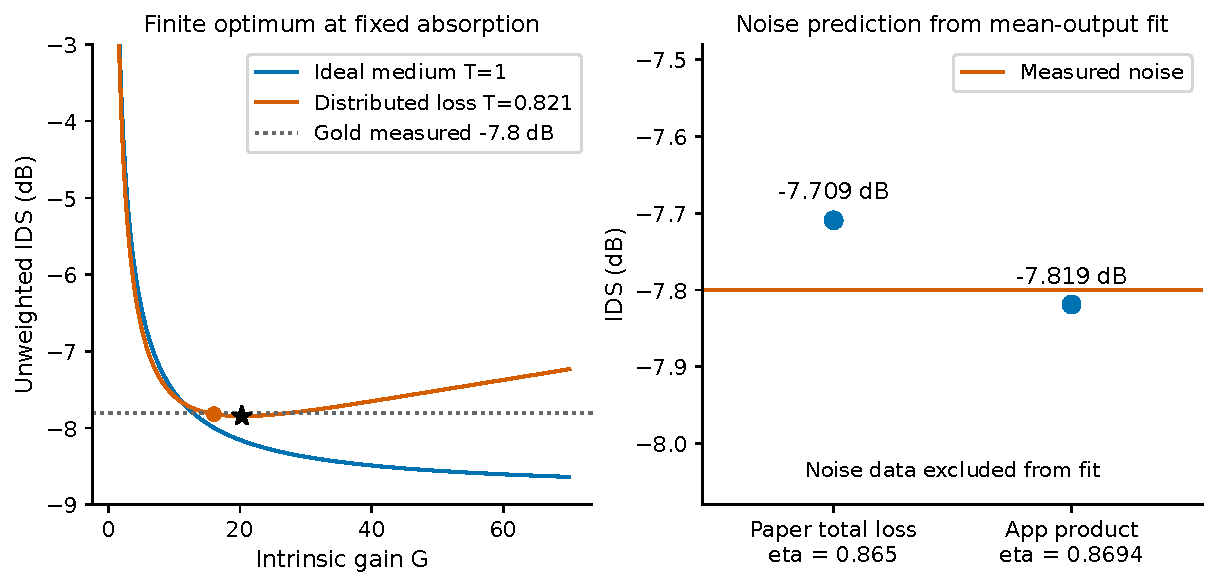
\includegraphics[width=.96\linewidth]{theory_gold_comparison.pdf}
\caption{Gold 평균 출력으로 제약한 분포모형, 이상적 손실모형과 실측 IDS.
분포모형은 스퀴징 값을 적합하지 않았다. 효율 정의와 반올림된 입력의
영향이 작은 잔차보다 클 수 있다.}
\label{fig:goldtheory}
\end{figure}

\subsection{고정하는 변수에 따른 최적점}
$\eta=.8694$, $w=1$에서 같은 분포모형에 세 가지 변화 방향을 적용했다.
표~\ref{tab:theoryopt}는 동일 함수의 서로 다른 단면이다.
실험의 온도 변화는 보통 이득과 흡수를 함께 바꾸므로, 고정 흡수의 최적
이득만으로 온도 최적점을 정할 수는 없다.

\begin{table}[htbp]\centering
\caption{분포모형의 조건부 최적점과 기준 $-7.819\dB$에서 $0.5\dB$ 이내인
연결구간. 모두 비가중 차분 $w=1$이다.}
\label{tab:theoryopt}
\begin{tabularx}{\linewidth}{P{4.4cm}P{3.1cm}Y}
\toprule 변화 방향 & 최적점 / IDS & $S\leq-7.319\dB$의 범위\\\midrule
내부 $G$; $T_s=.82116$ 고정 & $20.25$ / $-7.845$ dB & $7.58\leq G\leq63.68$\\
투과도 $T_s$; $G=16.026$ 고정 & $.93092$ / $-8.097$ dB & $.74697\leq T_s\leq1$\\
공통계수 $r\to xr,\ a\to xa$ & $x=1.0034$ / $-7.819$ dB & $.8037\leq x\leq1.2042$\\
\bottomrule
\end{tabularx}
\end{table}

고정 $T_s$에서 이득을 올리면 처음에는 쌍 상관이 커지지만, 이후에는
분포 흡수로 유입된 잡음의 재증폭이 불리하게 작용한다. 이 경쟁이 유한한
최적 $G$를 만든다. 고정 $G$에서 약간의 probe 흡수가 최적인 것은
비가중 차분에서 두 출력의 불균형과 분포 잡음이 함께 작용한 결과다.
이는 검출 전에 손실을 추가하라는 일반적 처방이 아니다.
외부 대칭손실은 식~\eqref{eq:ideal}에서 일관되게 IDS를 악화시킨다.

공통계수 $x$는 국소계수를 고정하고 셀 길이나 광학 깊이를 바꾸는 근사다.
기준 $x=1$이 최적점에 가까워, 단순한 이득 증가보다 이득과 흡수의 비를
개선하는 편이 유리하다. 온도는 Doppler 폭·충돌·population도 바꾸므로,
$x$의 약 $\pm20\%$ 범위를 그대로 온도 허용범위로 해석하지 않는다.

\begin{figure}[htbp]\centering
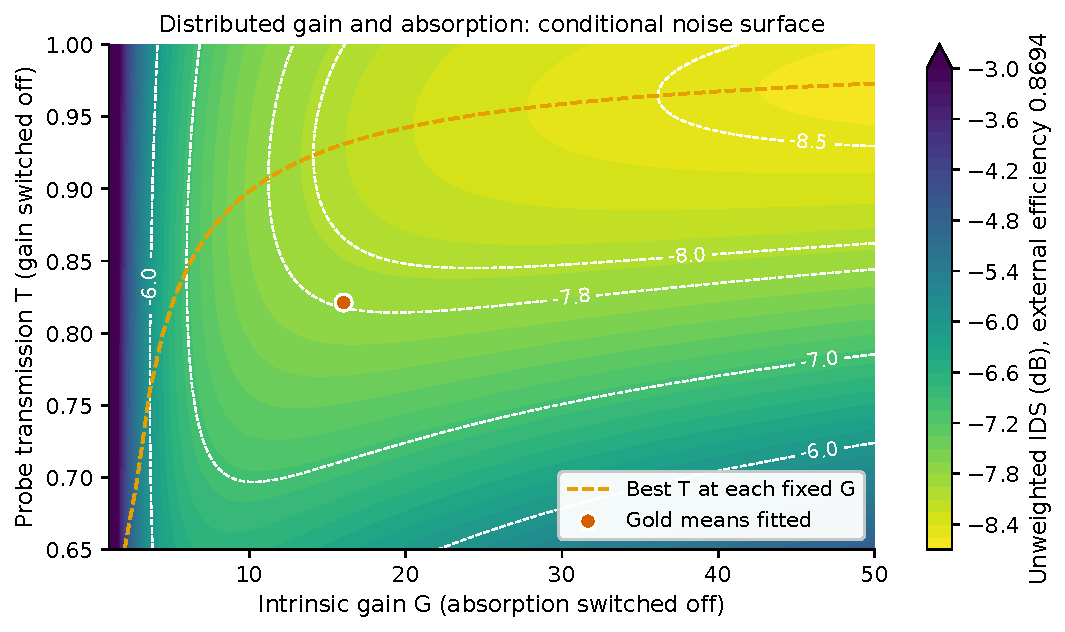
\includegraphics[width=\linewidth]{theory_gain_absorption.pdf}
\caption{내부 이득과 probe 흡수가 만드는 스퀴징 함수 및 단면.
표시된 이변수 영역의 최소는 이득 상한 경계에 있다. 표~\ref{tab:theoryopt}의
유한 최적점은 고정 흡수 또는 공통계수 변화라는 조건에 의존한다.}
\label{fig:ga}
\end{figure}

\subsection{손실·배경·seed 잡음의 공통 예산}
이상적인 동효율·비가중 검출에서 입력 seed의 초과 잡음을 $\xi$로 둔다.
이는 선택한 분석 주파수에서 입력 seed의 잡음 PSD/SNL$-1$이며,
해당 검출 대역의 초과 Fano factor에 대응한다. 독립 배경광을 제외한
twin-beam SNL로 정규화한 가산 잡음을 $\epsilon$이라 하면
\begin{equation}
 R=1-\eta+\eta\frac{1+\xi}{2G-1}+\epsilon.
 \label{eq:budget}
\end{equation}
쌍과 독립적인 coherent 광이 검출 총 SNL의 비율 $f$를 차지하면
$R_{\rm mix}=(1-f)R+f$다. $\epsilon$은 잡음 PSD의 비이고,
$f$는 총 SNL에 대한 기여비로 서로 다른 양이다.

\begin{table}[htbp]\centering
\caption{이상적 기준 $G=15,\eta=.8694,S_0=-7.943\dB$에서의 단일변수 예산.
다른 변수는 기준값으로 고정한다. 각 열의 상한을 동시에 사용할 수 없다.}
\label{tab:budget}
\begin{tabularx}{\linewidth}{P{5.2cm}YY}
\toprule 조건 & $+0.5\dB$ 이내 & $-7.8\dB$ 이하 유지\\\midrule
검출효율 $\eta$ 하한 & $0.84911$ & $0.86383$\\
이득 $G$ 하한 & $9.269$ & $12.794$\\
가산 잡음 $\epsilon$ 상한 & $0.019594$ SNL & $0.005379$ SNL\\
위 가산 잡음의 dB 값 & $-17.08\dB$ SNL & $-22.69\dB$ SNL\\
독립 coherent 광의 총 SNL 비율 $f$ & $2.334\%$ 이하 & $0.641\%$ 이하\\
입력 seed 초과 Fano factor $\xi$ & $0.654$ 이하 & $0.179$ 이하\\
전자차분 가중치 $w$ & $0.9822$--$1.0908$ & $0.9943$--$1.0776$\\
\bottomrule
\end{tabularx}
\end{table}

$-7.8\dB$ 유지에 쓸 수 있는 손실 여유는 총효율로 약 $0.557$
percentage point뿐이다. 배경광·전자 잡음·seed RIN이 공존하면 같은
여유를 나눠 쓴다. 국소적으로
\begin{equation}
 \delta R\simeq-\frac{2\eta}{(2G-1)^2}\delta G
 -\left(1-\frac1{2G-1}\right)\delta\eta
 +\frac{\eta}{2G-1}\xi+\epsilon+(1-R_0)f
\end{equation}
를 공통 상한과 비교한다. 변수마다 최대 공차를 배정한 직육면체는 일반적으로
전체 허용영역에 포함되지 않는다.

두 신호의 지연차도 상관을 낮춘다. 평탄한 실수 공분산을 가정하면
식~\eqref{eq:weighted}의 $C_{sc}$를 $C_{sc}\cos(\Omega\tau)$로
치환할 수 있다. Gold 이상기준에서 $500\kHz$를 평가하는 예로,
$0.5\dB$ 예산은 약 $12.6$ ns, $-7.8\dB$ 유지는 약 $6.6$ ns 이하의
잔여 지연차에 해당한다. 실제 공분산과 군지연 분산은 주파수별로 평가해야 한다.

\begin{figure}[htbp]\centering
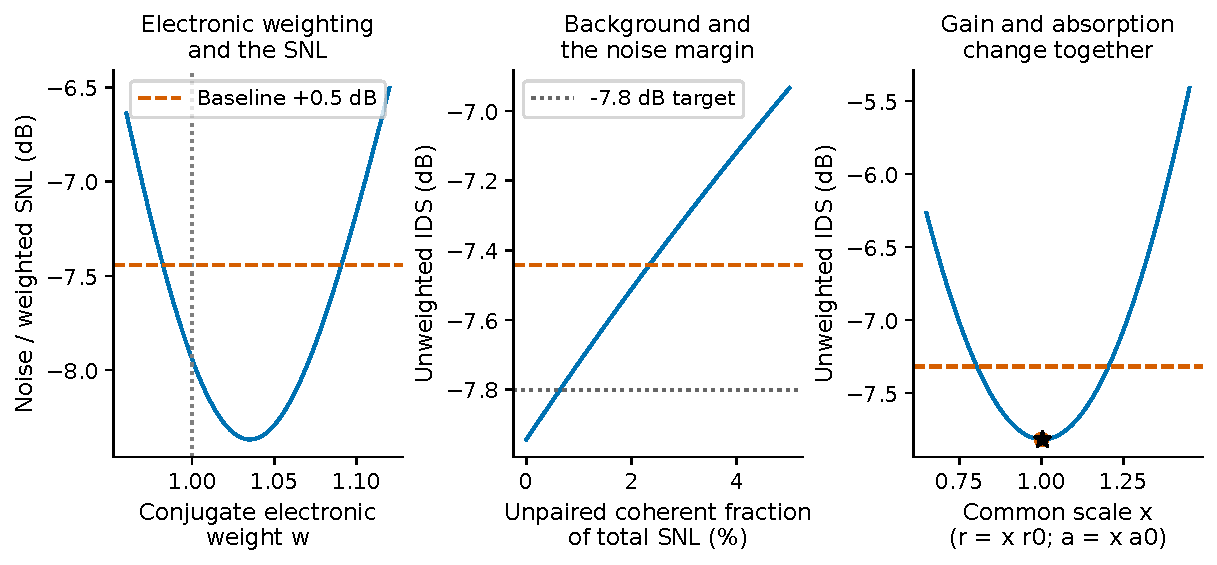
\includegraphics[width=\linewidth]{theory_tolerance.pdf}
\caption{이상적 검출모형의 잡음 예산과 분포모형의 민감도.
단일변수 상한은 공유 예산이다. 두 모형의 $0.5\dB$ 조건은 각각의 기준 IDS에
대한 것으로, 동일한 절대 임계값은 아니다.}
\end{figure}


\subsection{최저 dB와 실제 운전 전선의 구분}
검출 floor 근처에서는 서로 다른 큰 gain이 거의 같은 dB로 보인다.
따라서 최저 dB 한 점과 낮은 온도·pump·흡수에서 목표 성능을 달성하는
운전 전선은 다른 최적화 문제다. 목표 $S_\star$와 허용 모델 영역
$\mathcal D$에 대해
\begin{equation}
 \mathcal A(S_\star)=\{\bm x\in\mathcal D:
 S_{\rm IDS}(\bm x)\leq S_\star\}
\end{equation}
를 정의하고, 이 안에서 온도·pump 파워·산란·제어 민감도의 비용벡터를
모두 더 줄일 수 없는 점들을 Pareto 전선으로 삼을 수 있다. 어떤 비용을
선택했는지, 다른 변수는 고정했는지 또는 재조정했는지를 함께 지정해야 한다.
모델과 입력이 조건부이면 이 집합과 전선도 조건부이다.

물리적 허용영역에는 단순한 양의 gain 이외에 상태의 trace·양성,
광장 commutator, noise source closure, 공분산 불확정성, 독립 수치 수렴과
선형화·pump 고갈의 적용 범위가 필요하다. 탐색창 끝이나 허용성 검사의
경계에 놓인 최저점은 확정된 내부 최적점이 아니다. 실험 운전 전선을
제시하려면 측정 오차와 모델 오차를 포함한 목표 달성 확률까지 검증해야 한다.

\section{실험변수의 물리적 결합}
\subsection{OPD--TPD: 공명 위치와 세기}
원거리 detuning·약한 포화 근사에서는 Raman 결합이
$\Omega_{\rm eff}\propto\Omega_p\Omega_s/\Delta$,
광시프트가 $\delta_{\rm AC}\propto|\Omega_p|^2/\Delta$로 변한다.
OPD를 바꾸면 결합 세기와 최적 TPD가 함께 움직인다. 광시프트를
국소적으로 유지하는 조건은
\begin{equation}
 \delta\ln P_p-2\delta\ln w_p-\delta\ln|\Delta|\simeq0
\end{equation}
이다. 다준위·Doppler 평균·강한 pump에서는 정량식은 아니지만,
TPD 고정과 재조정에서 허용범위가 달라지는 원인을 설명한다.

\subsection{Pump 파워--빔 반경}
Gaussian beam의 중심 강도와 Rabi 주파수는
\begin{equation}
 I_{p,0}=\frac{2P_p}{\pi w_p^2},\qquad
 |\Omega_p|\propto\frac{\sqrt{P_p}}{w_p}.
\end{equation}
Gold 중심 강도는 약 $136\,\mathrm{W/cm^2}$이다. 국소 drive를
보존하는 일차 보상은 $\delta P_p/P_p\simeq2\delta w_p/w_p$다.
그러나 반경은 교차영역, 수집률, 원자 통과시간, Rayleigh 길이
$z_R=\pi w_p^2/\lambda$도 바꾼다. 같은 강도가 같은 IDS를 보장하지 않는다.

\subsection{온도--셀 길이}
광학 깊이의 주요 인자는 $\mathrm{OD}\propto N(T)L$이다.
밀도 증가는 이득을 높이지만 흡수·충돌·형광도 늘린다.
일정한 광학 깊이의 국소 조건은
\begin{equation}
 \delta\ln L\simeq-\frac{d\ln N}{dT}\delta T.
\end{equation}
코드의 증기밀도식은 $121\degC$에서 $d\ln N/dT\simeq0.05836$
K$^{-1}$, 온도 1°C 상승에 약 $5.99\%$ 밀도 증가를 준다.
같은 $NL$이어도 Doppler 폭·충돌률은 다르고, 셀 길이는
$\Delta k_zL$과 beam walk-off를 바꾼다. 온도와 길이는 주요 보상변수지만
완전히 하나의 곱으로 환원되지는 않는다.

\subsection{교차각--RF 평가 주파수}
등방 원자속도의 성분 표준편차 $\sigma_v=\sqrt{k_BT/m}$에 대해,
두 광장의 Raman Doppler 폭은
\begin{equation}
 \sigma_{\delta_\nu}=\frac{\sigma_v}{2\pi}
 \sqrt{(k_p-k_s\cos\theta)^2+(k_s\sin\theta)^2}.
 \label{eq:angle}
\end{equation}
Gold에서는 약 $1.380\MHz$로, 횡방향 성분이 약 $1.380\MHz$,
축방향이 약 $5.85\kHz$이다. 공선에서도 광주파수 차로 약 $1.99\kHz$가
남는다. 이는 RMS 폭이며 스퀴징 FWHM이나 허용 TPD 폭은 아니다.
작은 각도는 운동 dephasing과 위상 불일치를 줄이지만 pump 산란의
공간분리를 어렵게 한다. Wu 등은 약 $0.3^\circ$에서 $0.5^\circ$로
넓혀 이득·대역 일부를 희생하고 저주파 pump 산란을 줄였다\cite{wu}.
최적 각도는 평가 RF와 pump 제거계에 결합된다.

\subsection{Seed--검출 배경--spectral purity}
이상적인 bright-seed 식의 정규화 IDS는 seed 파워와 무관하다.
실제로 약한 seed에서는 고정 전자 잡음의 상대 기여가 커지고, 강한 seed에서는
원자 포화·pump 고갈·기술잡음이 증가한다. 국소 근사
\begin{equation}
 R(P_s)\simeq R_q+\frac{A_{\rm el}}{P_s}+B_{\rm tech}P_s,\qquad
 P_{s,*}=\sqrt{A_{\rm el}/B_{\rm tech}}
\end{equation}
는 양쪽 한계가 생기는 이유를 보여준다. 계수는 장치와 RIN에 의존하므로
미측정 계수를 넣어 gold의 최적 seed를 수치화하지 않는다.
EOM carrier와 불필요 sideband는 셀에서 각기 다른 증폭·흡수를 겪는다.
셀 입력의 불필요 광 비율을 표~\ref{tab:budget}의 검출면 비율 $f$로
직접 대체해서는 안 된다.

\section{GABES의 다변수 조건부 예측}
\subsection{평균장과 계산 조건}
GABES는 4준위 Bloch 계의 finite-seed Floquet 응답을 속도 평균하고,
probe--conjugate Maxwell 전파를 구한다. 원자상태는 $\Tr\rho=1$이며
열평형 population을 외부에서 중복 적용하지 않는다. Transit reset은
\begin{equation}
 \mathcal L_t\rho=\gamma_t(\rho_{\rm th}\Tr\rho-\rho),\quad
 \rho_{\rm th}=\operatorname{diag}(5/12,7/12,0,0),\quad
 \gamma_t=2\pi\times100\kHz
\end{equation}
로 두었다. 외부 결합에는 구조계수 $1/12$와 residual $\ell$이 들어간다.
$\ell$은 독립 측정된 원자상수가 아닌 유효계수다.

전파에는 주파수별 vacuum 파수와 기하학적 위상 불일치를 쓴다.
대칭 mismatch gauge의 장
$(E_se^{-\ii\Delta k_zz/2},E_c^*e^{+\ii\Delta k_zz/2})^T$에 대해
\begin{equation}
 M_E=\begin{pmatrix}
 \ii k_s\chi_{ss}/2-\ii\Delta k_z/2&\ii k_s\chi_{sc}/2\\
 -\ii k_c\chi_{cs}^*/2&-\ii k_c\chi_{cc}^*/2+\ii\Delta k_z/2
 \end{pmatrix},\quad \Delta k_z=2k_p-(k_s+k_c)\cos\theta .
\end{equation}
$k_j=\omega_j/c$이고 $\chi$는 무차원 물리적 감수율이다. 감수율의
분산은 위상 불일치에 다시 넣지 않는다. Ultra는 64구간의 교차 profile과
근사적인 pump-budget 감소를 포함한다.

이 절의 저장된 탐색 데이터는 gold 조건, 표준 red-seeded branch, Ultra, $N_F=3$을 썼다.
계산 계약과 소스 해시는 부록의 원본 배열에 결합되어 있으며, 다른 원자·잡음 모델의 결과로 재해석하지 않는다.
속도 간격은 5 m/s, cutoff는 $4\sigma_v$이며, TPD
$-80$--$120\MHz$를 $2\MHz$ 간격으로 스캔했다. 각 scan의 전체 구간에서
$N_F=2$와 비교하여 주 분석의 206개 scan 모두 Floquet 수렴 판정을 통과했다.
기준과 허용경계의 추가 정밀화는 2.5 m/s, $5\sigma_v$를 사용했고, 145회
평가 모두 판정을 통과했다. Gold gain은 정밀화로 약 $0.0087\%$,
조건부 IDS는 약 $0.000073\dB$ 변했다. 이는 선택한 일차원 모델 내부의
수치 검사다.

\subsection{Gold 이득의 일점 보정}
기본 $\ell=.74$는 gold에서 $G_s\simeq394.3$, $G_c\simeq396.5$를
주어 실측 $G_s\simeq15$보다 약 26배 크다. 이에 \textbf{probe 이득 15
한 개만} 이용하여 $\ell=0.42505$로 보정했다. 그러면
$G_s=15.000$, $G_c=14.157$이다. 스퀴징과 다른 운전점의 값·기울기는
보정에 사용하지 않았다. 다음 식을 GABES 그림의 목적함수로 삼았다.
\begin{equation}
 S_{\rm cond}(\bm x)=10\log_{10}
 \left[1-\eta+\frac{\eta}{2G_s^{\rm GABES}(\bm x;\ell_*)-1}\right],
 \qquad G_s^{\rm GABES}\geq1.
 \label{eq:conditional}
\end{equation}
이 환산은 $G_c=G_s-1$인 이상적 상관을 가정한다. GABES의 실제 $G_c$에서
원자 공분산을 계산한 값은 아니다. $G_s<1$인 수동영역에는 적용하지 않는다.
기준은 $S_0=-7.943\dB$, 허용 임계값은 $S_0+0.5=-7.443\dB$다.


\subsection{일점 보정의 외삽 범위}
전체 residual $\ell_*$을 맞춘 위 탐색과 별도로, 두 비대각 감수율에만
$C_{\rm mix}=0.5594938027$를 곱하는 평균장 보정이 있다.
이 계수는 Sim의 대표 probe gain 15.5에 맞추고 대각 감수율·검출손실·
원자상태는 그 보정에서 직접 바꾸지 않는 계약이다. 따라서
$\ell_*=0.42504822$와 같은 계수로 교환할 수 없다. 표~\ref{tab:frozenmix}는
$C_{\rm mix}$를 고정한 조건별 비교다. 이 자료의 평균장 계산은
pole 응답, Ultra 전파, 속도 간격 1 m/s와 $4\sigma_v$ cutoff,
64개 종방향 overlap 구간 및 출력 pump cap을 사용한다. 두 비대각 항에
동일한 상수를 곱하며, 빔 반경으로 변하는 별도 mixing 계수는 사용하지 않는다.
감수율의 변경에 상응하는 미시적 확산을 유도한 양자모형은 아니다.

Sim의 조건은 표~\ref{tab:gold}와 같다. Liu의 입력은
$(\Delta_\nu,\delta_\nu,T)=(0.8\GHz,-4\MHz,120\degC)$,
pump/seed 400 mW/10 $\mu$W, 반경 550/300 $\mu$m,
길이 12 mm, 교차각 $0.4^\circ$다. McCormick의 입력은
$(0.8\GHz,-4.267561\MHz,110\degC)$,
400 mW/100 $\mu$W, 반경 650/350 $\mu$m,
길이 12.5 mm, 교차각 $0.3^\circ$다. 이는 해당 문헌 비교에 사용한
명시적 입력이며 모든 apparatus 입력을 독립 측정했다는 뜻은 아니다.
\begin{table}[htbp]\centering
\caption{고정 비대각 보정계수의 probe power gain 비교. Sim은 적합점이며,
나머지는 계수 적합에 쓰지 않은 열람된 문헌 조건이다. 미열람 blind holdout이 아니다.}
\label{tab:frozenmix}
\begin{tabularx}{\linewidth}{P{3.4cm}rrrY}
\toprule 조건 & 문헌 & 보정 미적용 & 보정 적용 & 판정\\\midrule
Sim & 15.5 & 394.299 & 15.500 & 적합으로 정한 일치\\
Liu & 8 & 127.577 & 6.445 & 약19.4\% 낮음\\
McCormick 2008 & 9 & 7.133 & 1.926 & 약78.6\% 낮음\\
\bottomrule
\end{tabularx}
\end{table}
한 계수는 Sim·Liu의 이득을 낮추지만 McCormick 조건의 차이를 크게 만든다.
문헌의 excited-state detuning 기준과 미확인 apparatus 입력도 남아 있으므로,
이 차이를 특정 원자 과정의 크기로 곧바로 분해하지 않는다. 다만 한 점의
gain 일치가 넓은 조건의 정확성을 보장하지 않는다는 결과는 명확하다.
같은 Sim 입력에서 온도만 116, 121, 126\,$^\circ$C로 바꾼
세 점의 보정 gain은 각각 5.305, 15.500, 61.018이다. 이 큰 온도
의존성은 모형의 조건부 추세이며, 실험 온도 scan으로 검증된 예측은 아니다.

\subsection{OPD--TPD와 온도의 결합}
그림~\ref{fig:maps} 왼쪽은 OPD--TPD 면, 오른쪽은 각 OPD·온도에서 TPD를
다시 맞춘 최소값이다. TPD 고정 단면에서 민감한 변수도 TPD를 바꾸면
이득이 큰 다른 지점으로 보상할 수 있다. 각 변수를 독립 공차로 취급하기
어려운 이유를 이 지도에서 확인할 수 있다.
\begin{figure}[htbp]\centering
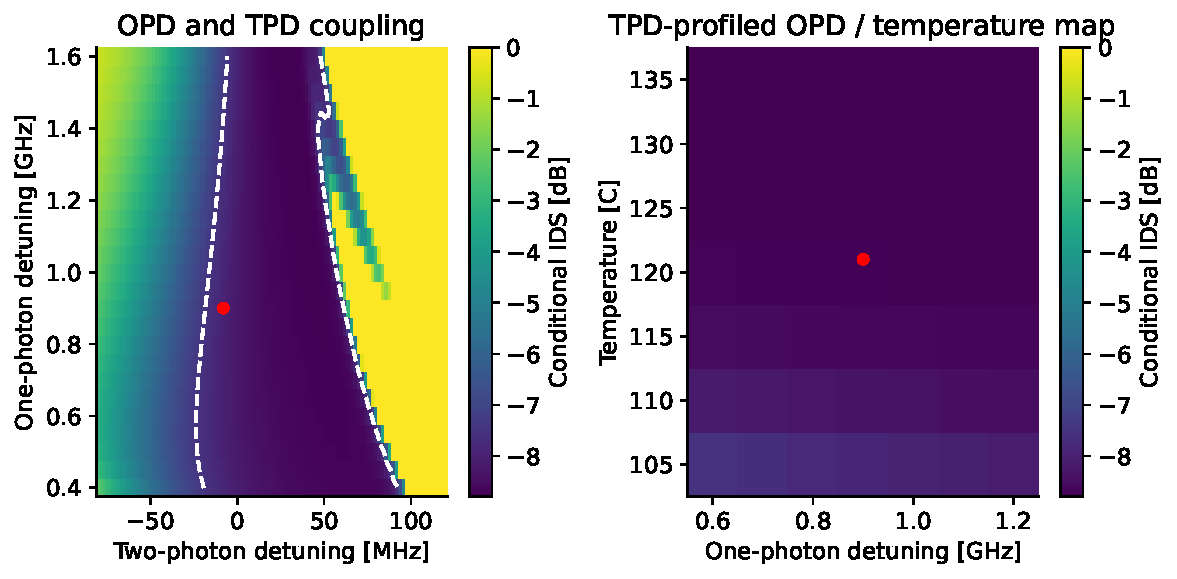
\includegraphics[width=\linewidth]{coupled_maps.pdf}
\caption{Gold 이득을 일계수로 보정한 GABES의 조건부 IDS.
왼쪽 흰 선은 $-7.443\dB$이고, 오른쪽은 TPD를 탐색 구간 안에서 재조정한다.
붉은 점은 gold 기준이다. 잡음은 식~\eqref{eq:conditional}로 환산한다.}
\label{fig:maps}
\end{figure}

다른 gold 변수를 고정하고 TPD를 정밀 탐색한 최소는
$\delta_\nu=46.25\MHz$, $G_s=222.10$, $S_{\rm cond}=-8.77582\dB$였다.
OPD $0.6$--$1.2\GHz$, 온도 $105$--$135\degC$의 이변수 주 격자에서는
$(1.2\GHz,135\degC,26\MHz)$가 $-8.83940\dB$로 최선이었다.
OPD·온도 모두 탐색 경계이므로 유한한 내부 최적점이 아니다.

이 고밀도 점은 small-signal gain 약 28,907에서 구간 pump 처리 후
약 18,457, 최종 cap 후 약 12,370으로 변한다. 마지막 cap만으로 약
33\% 감소한다. 반면 gold 기준의 최종 cap 영향은 약 0.035\%이다.
높은 이득의 지도 최소는 이상적 손실 floor $-8.84057\dB$에 접근한 결과로,
실험 운전점을 지시하지 않는다. 분포 잡음을 넣은 표~\ref{tab:theoryopt}의
유한 최적점과는 최적화하는 함수가 다르다.

\subsection{단일변수 허용폭과 TPD 재조정}
각 허용구간은 gold 기준점을 포함하고
$S_{\rm cond}\leq S_0+0.5\dB$인 \textbf{연결구간}이다.
재조정 TPD에도 같은 gold 임계값을 적용했다. 각 재조정점의 최소값에
별도로 $0.5\dB$를 더하지 않았다.
\begin{figure}[htbp]\centering
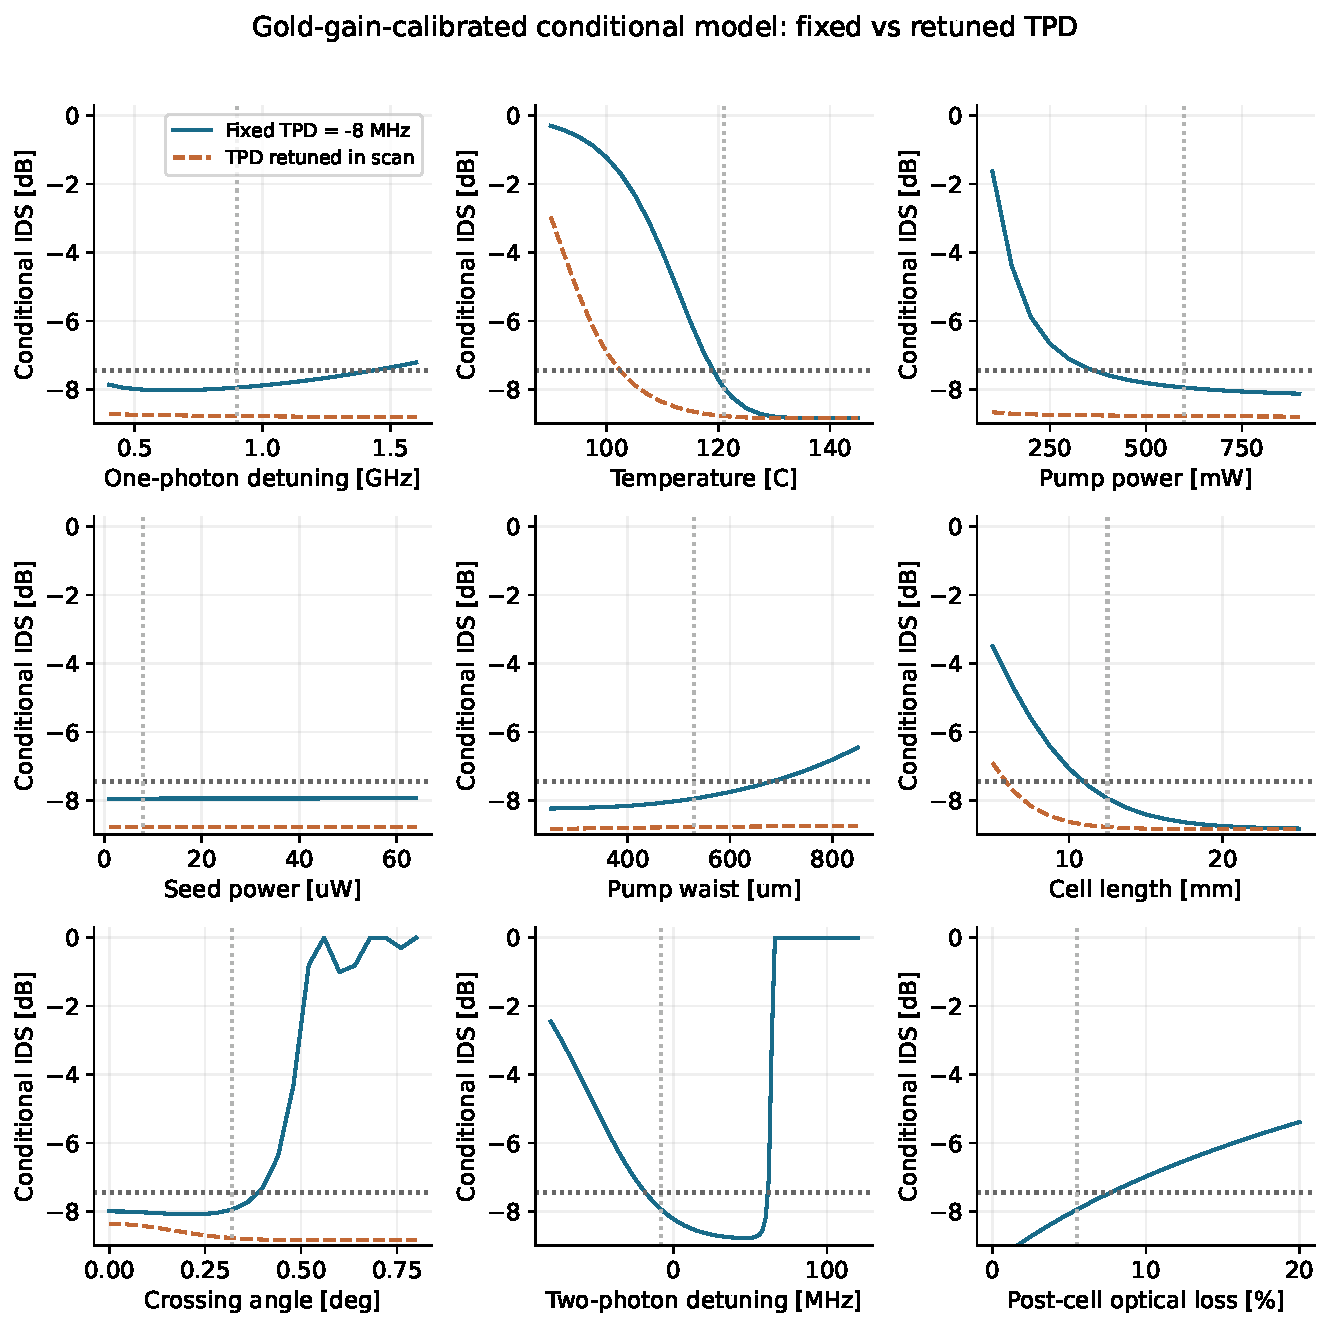
\includegraphics[width=.99\linewidth]{tolerance.pdf}
\caption{TPD $-8\MHz$ 고정(청색)과 탐색 구간 내 재조정(주황)의 단일변수
조건부 IDS. 수평 점선은 공통 임계값, 수직 점선은 gold 기준이다.
Seed의 평탄성과 높은 이득 쪽의 포화는 이상적 잡음 환산의 성질을 반영한다.}
\label{fig:tol}
\end{figure}

\begin{table}[htbp]\centering\small
\caption{조건부 $0.5\dB$ 허용구간. ``끝''은 탐색 끝에 걸렸다는 뜻이며
물리적 한계를 찾은 값이 아니다. 고정 TPD 교차경계는 세분화했고,
재조정 구간은 주 격자의 보간 근사다.}
\label{tab:codetol}
\begin{tabularx}{\linewidth}{P{3.1cm}P{2.8cm}P{4.2cm}Y}
\toprule 변수(기준) & 탐색범위 & TPD 고정 허용구간 & TPD 재조정\\\midrule
OPD ($.90\GHz$) & $.40$--$1.60$ & $.40$ (끝)--$1.4327$ & 전체 탐색범위\\
온도 ($121\degC$) & $90$--$145$ & $119.037$--$145$ (끝) & 약$102.4$--$145$ (끝)\\
Pump ($600$ mW) & $100$--$900$ & $361.84$--$900$ (끝) & 전체 탐색범위\\
Seed ($8\,\mu$W) & $1$--$64$ & 전체 탐색범위 & 전체 탐색범위\\
Pump 반경 ($530\,\mu$m) & $250$--$850$ & $250$ (끝)--$682.88$ & 전체 탐색범위\\
셀 길이 ($12.5$ mm) & $5$--$25$ & $10.898$--$25$ (끝) & 약$5.88$--$25$ (끝)\\
교차각 ($.32^\circ$) & $0$--$.8$ & $0$ (끝)--$.39053$ & 전체 탐색범위\\
외부 광학손실 ($5.5\%$) & $0$--$20\%$ & $0$--$7.71\%$ & QE $=.92$ 고정\\
\bottomrule
\end{tabularx}
\end{table}

TPD 자체는 다른 변수를 모두 고정한 상태에서
\begin{equation}
 -18.409\MHz\leq\delta_\nu\leq61.545\MHz
\end{equation}
가 허용 연결구간이다. 기준 $-8\MHz$ 대비 허용 drift는
$-10.409/+69.545\MHz$로 비대칭이다. 기준이 이 목적함수의 최적점이
아니기 때문에 대칭 공차로 바꾸면 정보를 잃는다.

이 모델에서는 온도를 낮추는 여유가 약 1.96°C로 작고, TPD를 함께 맞추면
허용영역이 크게 달라진다. Pump와 빔 반경은 강도 방향으로 결합하고,
각도도 TPD 보상을 받는다. 반면 seed $1$--$64\,\mu$W를 모두 허용하는
결과는 검출 배경과 포화의 실제 한계를 충분히 포함하지 못한다.
또한 출력 gain의 하한 처리가 수동영역을 $G_s=1$로 올리는 구간이 있어,
그림의 0 dB 평탄부를 실제 원자 잡음 예측으로 읽지 않는다.

\subsection{동시 drift와 제어 가능한 방향}
근방의 함수는
\begin{equation}
 S(\bm x_0+\bm u)\simeq S_0+\bm g^T\bm u+\tfrac12\bm u^TH\bm u
\end{equation}
로 전개된다. 기준이 최적점이 아니면 일차항 때문에 상·하한이 비대칭이다.
외란 $\bm u$와 조절변수 $\bm v$를 구분하고, 조절 방향이 국소 최적이며
$H_{vv}$가 양정치라면 재조정 후 곡률은
\begin{equation}
 H_{\rm prof}=H_{uu}-H_{uv}H_{vv}^{-1}H_{vu}
\end{equation}
이다. TPD 추종으로 허용영역이 넓어지는 효과가 교차항에 대응한다.
이번 다봉형 scan은 직접 최소화를 사용했으며, 하나의 Hessian으로
넓은 범위를 외삽하지 않았다. 먼 TPD 가지로의 이동에는 실제 lock이
연속적으로 따라갈 수 있는지도 추가 검증해야 한다.

\section{문헌과 이론의 정량 비교}
\subsection{동일 관측량으로 비교할 수 있는 실험}
\code{references/fwm_squeezing_paper_parameters.csv}의 10개 논문을
출발점으로 측정방식·손실정의·운전점을 일차자료에서 확인했다.
표~\ref{tab:direct}는 실측 이득과 총효율이 비교적 명확한 직접 IDS 세 사례다.
각 실험의 값을 식~\eqref{eq:ideal}에 대입한 결과다.
\begin{table}[htbp]\centering
\caption{실측 이득을 입력한 이상적 손실식의 IDS 비교.
잔차는 실측 minus 계산이다. 원자 이득의 독립 예측을 평가하는 표는 아니다.}
\label{tab:direct}
\begin{tabularx}{\linewidth}{P{3.6cm}P{2.4cm}P{2cm}P{2.8cm}Y}
\toprule 문헌 & $G$, $\eta$ & 실측 dB & 계산 dB & 잔차 dB\\\midrule
Sim 2025\cite{sim} & $15$--$16$, $.865$ & $-7.8$ & $-7.830$--$-7.881$ & $+.030$--$+.081$\\
McCormick 2007\cite{mc07} & $4$, $.656$ & $-3.5$ & $-3.588$ & $+.088$\\
McCormick 2008\cite{mc08} & $9$, $.90$ & $-8.0$ & $-8.155$ & $+.155$\\
\bottomrule
\end{tabularx}
\end{table}

차이는 약 $0.03$--$0.16\dB$로, 직접 IDS의 규모는 이득과 손실로 잘
설명된다. 각 숫자가 반올림되어 있고 공통된 통계 오차모형이 없으므로
잔차를 예측오차 분포나 신뢰구간으로 삼지 않는다.
특히 McCormick 2008의 원논문은 분포 이득·흡수를 사용해 내부
$G\simeq9$--$15$, 투과도 $T_s\simeq.85$--$.95$ 영역을 비교한다.
유효 출력 gain 9를 간단한 식에 넣는 것은 이 처리의 근사다.

Gold 분포모형은 평균 출력 두 개로 이득과 흡수를 분리하고,
식~\eqref{eq:cov}를 통해 잡음을 예측했다는 추가 의미가 있다.
다음 검증은 같은 계수로 다른 온도·detuning·pump를 예측하는 것이다.
그때 보정점 바깥에서의 모델 성능을 평가할 수 있다.


Pooser 등\cite{pooser}은 Rb 동위원소와 D1/D2 전이를 비교하여 이득과
상관 생성의 계 의존성을 조사했고, Jasperse 등\cite{jasperse}은 분포
이득·손실을 실험 진단에 사용하는 해석 모형을 제시했다. 이런 자료는
원자종·전이·검출 조건을 바꾸었을 때의 모형 범위를 정하는 데 유용하다.
서로 다른 전이·검출량의 최고 dB를 하나의 예측오차 표에 합치지는 않는다.

\subsection{다른 레퍼런스에서 드러나는 물리}
\begin{table}[htbp]\centering\small
\caption{추가 참조실험의 측정방식과 모델에 주는 제약.}\label{tab:others}
\begin{tabularx}{\linewidth}{P{3.05cm}P{3.05cm}Y}
\toprule 문헌 & 주요 결과 & 이론과 대응 및 비교 범위\\\midrule
Vogl 2012\cite{vogl} & 직접 IDS $-2.1\dB$, gain $4$--$10$ &
Blue seed를 쓰는 다른 Raman branch. 총효율이 없고 red-seed 코드의
동일 회귀 대상으로 볼 수 없다. Compact 구성과 모드 수집의 참고 사례.\\
Liu 2011\cite{liu} & 직접 IDS 약 $-5\dB$, gain 약8 &
QE $.96$만 넣으면 이상식은 $-9.83\dB$다. 광학손실 정보가 부족하므로
차이 $4.83\dB$ 전부를 원자 잡음으로 볼 수 없다. Pump $100\to700$ mW에서
SQL 교차대역이 $5.5\to16.5\MHz$로 변한다.\\
Wu 2019\cite{wu} & Dual seeding, 20 Hz 이상에서 5 dB 초과, 10 Hz 미만 sub-shot &
단일 seed의 gain과 최종 dual-seed IDS를 섞지 않는다.
공통 기술잡음, pump 산란과 각도·저주파 특성의 관계를 제공한다.\\
de Araujo 2024\cite{araujo} & Homodyne quadrature 4 dB 초과, sub-1 Hz &
Vacuum seed와 LO를 쓰므로 직접 IDS식과 같은 dB 비교가 아니다.
군지연 보상·LO 공간모드·공분산 평가에 유용하다.\\
Allen 2026\cite{allen} & 직접 IDS 최고 $-8.2\dB$, 장시간 평균 약 $-7.905\dB$ &
Seed·pump·cell·etalon 온도의 실측 scan과 안정화 정보를 제공한다.
다음 절에서 실험 기반 tolerance로 사용한다.\\
Jain 2025\cite{jain} & Fiber 전 $-7.2\dB$, 후 $-4.4\dB$ &
10\% 대칭 vacuum 손실만 가정하면 $-5.662\dB$다.
관측은 추가 $1.262\dB$ 악화하여 모드선택·불균형 잡음의 설명이 필요하다.\\
Monsa 2026\cite{monsa} & Compact 계, pump 약300 mW, IDS 약 $-8\dB$ &
Preprint 결과. 총효율과 잡음보정 정의가 충분히 정합되지 않아
정밀 보정보다 장치 구성의 참고로 사용한다.\\
\bottomrule
\end{tabularx}
\end{table}

Jain의 fiber 사례는 높은 파워 결합효율만으로 쌍의 공간상관이 보존되지는
않는다는 점을 보여준다. $R_{\rm before}=10^{-7.2/10}$에 정확히 10\%의
대칭 vacuum 손실을 적용하면
\begin{equation}
 R_{\rm vac}=.9R_{\rm before}+.1=0.27149,\qquad
 10\log_{10}R_{\rm vac}=-5.662\dB.
\end{equation}
실측 후 $R=10^{-4.4/10}=0.36308$과 차이는 약 $0.0916$ SNL이다.
이것은 명시된 손실 가정 아래의 부족분으로, 한 원인에 전부 귀속한 측정이 아니다.

총효율이 없으면 $\eta_{\rm inv}=(1-R_{\rm exp})/[1-(2G-1)^{-1}]$를
역산할 수 있다. Liu는 약 $.733$, Monsa는 약 $.872$다.
하지만 이 값은 미지의 손실·불균형·기술잡음을 합친 실효값이며 측정효율이 아니다.
이를 다시 IDS 예측에 넣는다면 독립 비교가 아니라 순환적인 맞춤이 된다.

\section{실측으로 확인한 운전 허용범위}
\subsection{Allen 실험의 변수 scan과 안정화}
Allen 등\cite{allen}은 셀 $118\degC$, OPD $950\MHz$, TPD $-1\MHz$,
pump $500$ mW, seed $12\,\mu$W 근방에서 변수를 조사했다.
표~\ref{tab:allen}은 이 장치와 다른 조건을 고정했을 때의 결과로,
gold에 바로 이식하는 공차는 아니다. 계산의 조건부 이득 scan과 실험
안정 운전의 차이를 판단할 직접적인 자료다.
\begin{table}[htbp]\centering
\caption{Allen 2026에서 실측한 조건부 허용영역과 제한.}
\label{tab:allen}
\begin{tabularx}{\linewidth}{P{2.6cm}P{4.3cm}Y}
\toprule 변수 & 관측 범위·안정도 & 물리 및 제어 의미\\\midrule
셀 온도 & $118\degC$ 주변 $\pm1\degC$에서 IDS 변화 작음 &
Conjugate 출력은 2°C 변화에 50 $\mu$W 초과, 약25\% 변한다.
IDS 안정과 파워 안정은 다른 사양이다.\\
Etalon 온도 & 최적 약 $26.95\degC$; $\pm2.5$ m°C 유지 &
Seed 투과와 불필요 모드 배제가 같이 변해 IDS·출력을 제한한다.\\
Seed 파워 & $12$--$20\,\mu$W IDS plateau &
약11 $\mu$W 미만에서는 검출배경 영향 증가, 20 $\mu$W 초과는
포화로 점진적 악화.\\
Pump 파워 & 측정범위 내 최상 IDS 약450 mW 이상; conjugate 최대 약500 mW 이상 &
눈에 띄는 변화에는 수십 mW를 요했고 수 mW의 안정도는 해당 운전점에서 충분했다.\\
레이저 주파수 & 10분 간격 재조정 &
원자 이득과 etalon 투과 모두 추종해야 한다.
레이저 단독의 공차로 환원되지 않는다.\\
\bottomrule
\end{tabularx}
\end{table}

재조정한 5시간 측정은 평균 $-7.905\pm.048\dB$, 시간 표준편차
$.103\pm.032\dB$였고, 재조정하지 않으면 평균 $-7.35\pm.23\dB$,
시간 표준편차 $.46\pm.15\dB$였다. 평균과 표준편차의 불확도는 원문
집계량을 인용했다. 주파수 탐색의 종료 폭 약 $11\MHz$는 알고리즘 설정이며,
측정된 IDS의 허용 레이저 drift 폭으로 읽지 않는다.

\subsection{함께 제어해야 하는 변수}
\begin{table}[htbp]\centering
\caption{결합변수와 실제로 추적할 관측량.}
\begin{tabularx}{\linewidth}{P{4.2cm}Y}
\toprule 결합변수 & 추적·제약할 양\\\midrule
OPD--TPD--pump 강도 & 광시프트에 의한 공명 이동과 두 출력·IDS를 동시 측정.\\
Pump 파워--빔 반경 & $P_p/w_p^2$뿐 아니라 중첩·원자 통과·수집모드.\\
온도--셀 길이--detuning & 이득 대 흡수의 비, 잡음바닥, 밀도변화의 보상 가능성.\\
교차각--pump 배제--RF & 위상정합·Doppler 폭과 산란배경을 같은 RF에서 비교.\\
Seed--etalon--레이저 & Seed 총파워, carrier/sideband 구성, 각 출력으로의 누설.\\
두 효율--전자 가중치--지연 & DC balance, 주파수별 cross spectrum과 같은 가중치의 SNL.\\
\bottomrule
\end{tabularx}
\end{table}

Gold의 잔여 carrier 실험에서 입력 carrier/seed $0.5\%$도 스펙트럼을
악화시켰다. 비율 $12.5\%$에서는 slope비 $.589$ ($-2.30\dB$),
$25\%$에서는 $.964$ ($-.159\dB$)였다\cite{sim}.
단지 sub-shot을 유지하는 것보다 $7$--$8\dB$ 영역의 spectral purity
요건이 엄격하다. 셀 앞 불필요 광의 합계뿐 아니라, 셀·필터 이후 그 광이
각 검출기의 SNL과 잡음에 기여하는 양을 알아야 한다.


\section{미시적 잡음 계산에서 확인한 범위}
\subsection{응답과 잡음을 함께 계산하는 기준}
평균 이득을 잡음으로 환산하는 대신, 명시한 Hamiltonian과 reservoir로
원자 상태를 구하고 그 상태의 상관함수를 계산할 수 있다. 사용한 기본식은
\begin{equation}
 \dot\rho=\mathcal L\rho=-\frac{\ii}{\hbar}[H,\rho]
 +\sum_r\left(L_r\rho L_r^\dagger-\tfrac12\{L_r^\dagger L_r,\rho\}\right).
\end{equation}
여기서 $L_r$는 자발방출·명시적 replacement 등 선택한 환경 채널이다.
원자 관측량의 connected fluctuation $\delta O_j=O_j-\langle O_j\rangle$에
대해 두 연산자 순서의 상관 $\langle\delta O_j(t)\delta O_k^\dagger(t')\rangle$와
$\langle\delta O_k^\dagger(t')\delta O_j(t)\rangle$를 각각 유지한다.
두 값의 차는 commutator와 관련되지만, 그 차만으로 두 잡음의 절대 크기를
정할 수는 없다. 응답으로부터 필요한 최소 잡음을 역산하여 실제 reservoir
잡음을 대신하지 않는다.

독립 양자회귀(quantum regression, QRT) 계산은 같은 물리적
$\mathcal L$에서 원자 density와 두 시간 상관을 직접 전파한다.
응답·확산의 축약 결과를 다시 입력하는 방식이 아니라, 독립적인
상관 전파와 비교하는 것이 검산이다. 광장으로 옮긴 뒤에는
진공 공분산 $I/2$와 $[x,p]=\ii$인 명시적 quadrature 순서에서
commutator, 완전양성 및 uncertainty를 확인한다. 부록의 미시적
자료는 이 기준으로 얻은 수치이며, 각 모델의 생략된 자유도까지
검증하는 것은 아니다.

\subsection{단일 속도에서의 조건부 readout}
표~\ref{tab:microreadout}는 reduced D1 원자 하나의 속도계급을 대표하는
균일매질 계산이다. Pump $600$ mW, 반경 $530\,\mu$m, 밀도
$10^{18}\,\mathrm{m}^{-3}$, 약한 장의 면적 $1.2\times10^{-7}$ m$^2$,
길이 12.5 mm, seed $8\,\mu$W, $\Delta_\nu=.9$ GHz,
$\delta_\nu=-8$ MHz, replacement rate $2\pi\times100$ kHz를 선언했다.
Pump는 Gaussian 중심 강도로 고정하고, 검출 응답은 평탄하며 전자잡음은
0으로 두었다. 이 조건의 density와 replacement rate는 별도 입력이며
실험 온도로부터 검증된 thermal stream을 만든 값이 아니다.

강도 평균을 재현하도록 정의한 양의 Zeeman RMS dipole을 pump·약한 장의
구동·편극 readout에 일관되게 적용했다. 이 평균 dipole은 약한 흡수의
manifold 평균을 보존하지만 실제 signed Clebsch--Gordan 경로와
편광 간 간섭, pump로 변한 Zeeman population을 복원하지 않는다.
\begin{table}[htbp]\centering
\caption{같은 조건부 원자 상태에서 얻은 gain과 IDS. 모든 열은 실험 예측이 아닌
명시한 단일 속도 모델의 출력이다.}\label{tab:microreadout}
\begin{tabularx}{\linewidth}{Yrrr}
\toprule 총 검출효율 & 0.1 MHz [dB] & 1 MHz [dB] & 4 MHz [dB]\\\midrule
$\eta_s=\eta_c=1$ & $-.873105$ & $-.872957$ & $-.870698$\\
$\eta_s=\eta_c=.85$ & $-.730416$ & $-.730294$ & $-.728436$\\
$\eta_s=\eta_c=.50$ & $-.414648$ & $-.414582$ & $-.413565$\\
\bottomrule
\end{tabularx}
\end{table}
Probe와 conjugate power gain은 각각 1.11065587과 0.11356221이며
검출효율을 바꾸어도 동일하다. 밀도 또는 길이를 0으로 두면 각각
$G_s=1$, $G_c=0$, $R=1$을 회복한다. SQL 한계의 절대 오차는
$1.11\times10^{-16}$, 대칭손실 법칙의 오차는 $3.33\times10^{-16}$이고,
모든 경우의 광장 channel 검사를 통과했다. 38개 소비 scalar를 assumed로
기록한 독립 입력 감사는 실패한다. 이 실패는 수치 오작동이 아니라
실측 입력의 근거가 없다는 정확한 표시다. 이 계산의 약 $-0.73\dB$를
뜨거운 증기 실측 $-7.8\dB$와 빼서 실험 예측오차로 보고하지 않는다.

\subsection{움직이는 원자와 열적 앙상블}
열 원자 경로 계산에서는 경계로 들어오는 flux가
\begin{equation}
 dJ=n f_T(\bm v)|\bm v\cdot\bm n_{\rm face}|\,dA\,d^3v
\end{equation}
를 따른다. 경계 state의 불확도, 경로 내부의 자발방출 잡음, 경계를
통과하는 원자 수의 Poisson 변동을 구별한다. 원자 경로를 직접 계산할 때
동일한 transit를 별도의 순간적인 thermal reset으로 다시 적용하지 않는다.
독립 Poisson 도착 경로의 스펙트럼은 경로별 raw second moment를 도착률로
가중하여 합한다. 평균 pulse를 먼저 위상 평균하여 0으로 만든 뒤
제곱하면 원자 수 변동의 항을 잃을 수 있다.

선택된 moving Rb 경로의 독립 QRT 검산에서 boundary 항을 제거하면
greater covariance norm이 18.06\%, 서로 다른 구간 사이의 covariance를
제거하면 333.46\% 바뀌었다. 따라서 순간적인 local noise만 더하는
계산은 일반적인 원자 수송과 같지 않다. 이 비율은 그 single-atom
fixture의 행렬 norm 변화이며 실험의 dB 오차가 아니다.

전체 열적 평균의 검증에는 각 경로의 정확성과 경로·속도 적분 수렴이
둘 다 필요하다. 표~\ref{tab:thermalpath}의 p2 표본 계산은
열린 정사각 기둥으로 유입되는 pump-only Gaussian reduced-Rb stream을
가정한다. 온도 $T=373$ K, 수밀도 $n=10^{18}\,\mathrm{m}^{-3}$,
기둥 길이 12.5 mm, 횡단면 한 변 $346.410\,\mu$m
(반폭 $173.205\,\mu$m)이며, pump는 600 mW, 반경 $w=530\,\mu$m다.
유입 원자는 무편극 바닥상태 혼합으로 두 초미세 준위의 점유율이
각각 $5/12$, $7/12$다. 횡방향 측벽에서 pump 세기는
$I(x,y)/I(0,0)=\exp[-2(x^2+y^2)/w^2]$에 따라
모서리의 약65.2\%에서 변 중앙의 약80.8\%다. 따라서 유입면은
pump가 사라지는 먼 cell 경계가 아니며, 이 경계 상태를 실제 cell의
광펌핑 이력으로 간주할 수 없다. RF는 0.1, 1, 4 MHz이고 세 독립 Sobol scramble의 24경로씩을
합하여 72개의 고유 경로를 다룬다. 각 경로에는 CF4 세 해상도와 독립
adjoint 두 해상도의 다섯 계산이 있다. finite seed·실제 cell의 pump history·
광장 nonlocal Maxwell 전파와 검출 SQL은 이 stream 계산에 포함하지 않는다.
\begin{table}[htbp]\centering\small
\caption{열적 경로 적분의 정확도와 앙상블 적분의 수렴은 별도 결과다.
경로 오차는 seed 811의 24경로 최대값이다.}\label{tab:thermalpath}
\begin{tabularx}{\linewidth}{P{7.1cm}YY}
\toprule 검사 & 관측값 & 기준 또는 상태\\\midrule
CF4 첫 / 둘째 refinement & $5.35\times10^{-6}$ / $2.13\times10^{-7}$ & 각각 $10^{-3}$ 통과\\
Finest CF4 대 독립 adjoint & $6.08\times10^{-8}$ & $5\times10^{-6}$ 통과\\
Adjoint 자체 refinement & $1.38\times10^{-7}$ & $2\times10^{-6}$ 통과\\
서로 다른 scramble의 전체 방향 비교 & 0/6 방향 통과 & 각 metric 5\% 이하 필요\\
선언한 격자 / 평가된 격자 & 9 / 3 & p3·p4 각 세 seed 미평가\\
고유 경로 / 완료한 원자 계산 & 72 / 360 & 전체 요청 1,440 중 360\\
검증된 격자 refinement edge & 0 & 전체 thermal 수렴 미인증\\
\bottomrule
\end{tabularx}
\end{table}

\begin{table}[htbp]\centering\small
\caption{p2 세 seed의 여섯 유향 비교에서 얻은 metric별 최대 상대 행렬 변화의 범위.
범위의 양 끝은 여섯 방향 중 최소·최대이며 신뢰구간이 아니다.}\label{tab:thermalscramble}
\begin{tabularx}{\linewidth}{P{8.0cm}Y}
\toprule Metric & RF/source 최대값의 방향별 범위\\\midrule
Greater / lesser 전체 & 12.86--19.90\% / 12.89--19.96\%\\
Greater / lesser source별 & 25.56--43.61\% / 22.17--43.33\%\\
Poisson number & 5.70--9.06\%\\
복소 retarded response & 25.78--34.37\%\\
\bottomrule
\end{tabularx}
\end{table}
각 비교의 분모는 기준 행렬의 Frobenius norm과 선언한 SI roundoff
scale 중 큰 값이다. 여섯 metric이 모두 기준 안에 들어야 한 방향이 통과한다.
상대 변화는 참 적분오차의 상계나 확률적 신뢰구간이 아니며, source나
seed를 평균하여 실패를 감추지 않는다. 점유수/$nV$도 각 seed에서
0.8302, 1.1103, 0.8561로 달라 사후 재정규화를 적용하지 않았다.
계산이 정확한 개별 경로를 많이 확보한 사실만으로 열적 적분은 인증되지 않는다.

\begin{figure}[htbp]\centering
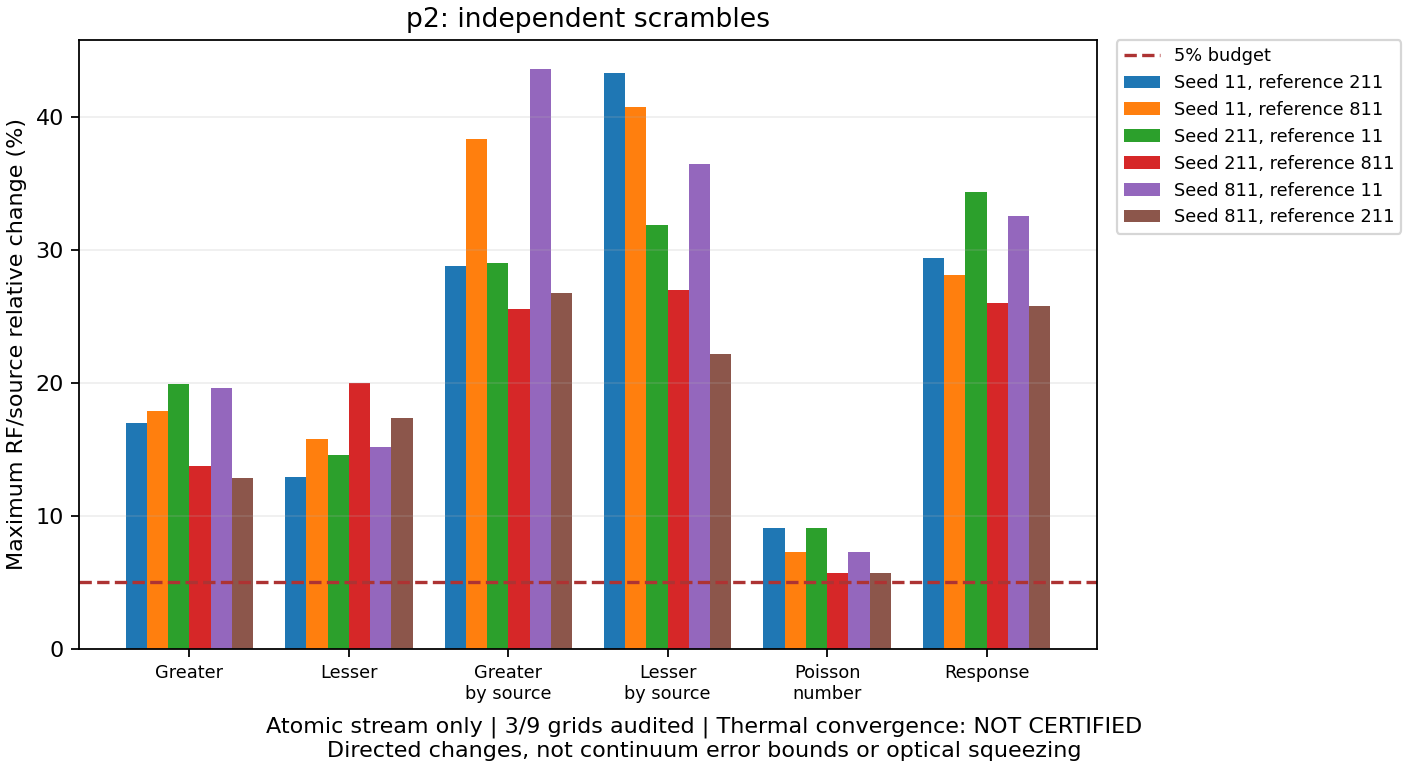
\includegraphics[width=\linewidth]{thermal_campaign_scrambles_p2_three_seeds_v2.png}
\caption{열적 p2 세 scramble의 여섯 유향 비교. 수평 기준선은 5\%다.
각 곡선은 같은 물리 조건의 quadrature 표본을 바꾼 결과이며, 다른
실험 detuning·온도·pump 조건에서의 예측 검증을 뜻하지 않는다.
그림과 복소 행렬은 고정된 캠페인 증거를 재사용했다.}
\label{fig:thermal}
\end{figure}

\subsection{현재 결과가 운전 전선에 주는 제약}
열적 행렬의 5.70--43.61\% 변화는 광학 IDS의 같은 비율 오차로
환산할 수 없다. 해당 원자 stream에 비국소 광장 전파와 동일 조건 SQL을
연결하지 않았기 때문이다. 원자 response와 noise가 수렴한 뒤 그
오차를 optical covariance와 검출 readout으로 전파해야 실제 dB 오차가 된다.
독립 scramble은 수치 적분 검산이고, 독립 실험 조건은 예측 검산이다.

그러므로 본문의 Gaussian 최적점은 해당 해석 모형의 최적점으로,
평균장 지도는 목표 gain에 조건을 둔 탐색으로 사용한다. 열 원자 전체의
microscopic gain·IDS·RF bandwidth를 이미 예측하는 것으로 승격하지 않는다.
소스·불확도·수렴이 갖춰진 결과에 한해서만 탐색 영역을 점진적으로 넓힐 수 있다.

\section{실험 예측과 운전영역을 검증하는 조건}
\subsection{미확정 입력과 모델 범위}
\begin{table}[htbp]\centering\small
\caption{실험 적용을 제한하는 조건과 필요한 관측량.}\label{tab:limits}
\begin{tabularx}{\linewidth}{P{3.0cm}Y Y}
\toprule 항목 & 현재 근거와 한계 & 필요한 판정\\\midrule
결합·평균 이득 & 기준 gain을 맞춘 두 종류의 유효계수는 독립 원자상수가 아니다.
고정계수의 다른 조건 비교도 큰 잔차를 남긴다. & 두 출력과 입력 seed를
동시에 측정하고 CG·편광·population·overlap·transit의 입력을 독립화한다.\\
미시적 원자 잡음 & reduced 모델의 응답·ordered noise 및 일부 광장 readout은
구현·검산됐다. 전체 thermal 광장 예측은 미완성이다. & 경로 및 앙상블 수렴,
nonlocal Maxwell, 양 순서 source closure·commutator·CP를 함께 검사한다.\\
이차원 운동과 공간모드 & Gold Raman RMS 약1.38 MHz, 정지 원자 고정 모드와
pump-only moving path가 별도 조건에서 검증됐다. & finite seed의 공간 수송,
diffraction·walk-off·추가 수집모드 및 velocity-changing collision을 제한한다.\\
Pump 고갈 & 구간 pump-budget과 최종 cap은 세 광장·원자의 자기일관 해가 아니다.
저장된 지도 최저점은 cap만으로 gain 약33\% 감소. & 위치별 세 mean field와
원자 state·응답·잡음 재계산, 에너지 수지 및 모드·공간격자 수렴이 필요하다.\\
RF와 기술잡음 & TPD 폭·Raman RMS·원자 pole·검출 roll-off는 RF IDS bandwidth와 다르다. &
팔별 PSD와 complex cross PSD, SQL/dark/transfer, RIN·산란·지연 및 대역 정의를 맞춘다.\\
측정면과 불확도 & Gold 효율 규약만으로 약0.11 dB 차이가 생긴다.
현재 assumed ledger는 no-fit 조건을 충족하지 않는다. & 원시 powers·독립 losses·
QE·측정일·적용 조건·공분산을 기록하고 예측구간에 전파한다.\\
\bottomrule
\end{tabularx}
\end{table}
펌프로 원자 상태를 다시 푸는 4준위 모형에는 그 모형이 허용하는
hyperfine population 재분배가 있다. 이를 ``정상상태이므로 광펌핑이 없다''고
분류하지 않는다. 남은 문제는 실제 signed Zeeman 경로·편광·충돌·수송과
모드의 충분성이다. 원자 generation의 CP 통과 또한 그 reservoir가
해당 실험을 충분히 묘사한다는 증명은 아니다.

\subsection{독립 입력과 미열람 실험 조건}
Waist를 독립 beam-profile 측정에 fit하거나 detector 전달함수를 별도
교정 trace에 fit하는 것은 독립 입력과 양립한다. 반대로 목표 FWM gain이나
IDS를 보고 waist·coupling·loss를 정하면 target-fitted 입력이다.
모든 소비 값에 단위·출처·불확도·적용 조건을 연결하고, 목표 데이터가
입력 추정에 들어갔는지 확인해야 한다. fitted라는 표시만으로 독립성을
승인하지 않는다. 현재 SABES 입력 85개 중 nominal 47개, lab 10개,
fitted 13개, paper 8개, datasheet 7개라는 분류는 자료의 출처 요약이며
독립 입력의 완성도나 실험 예측 정확도를 뜻하지 않는다.

검증 데이터는 하나의 RF trace에서 bin을 일부 숨기는 방법 대신,
$\Delta_\nu,\delta_\nu,T,P_p,P_s$와 geometry의 운전조건 전체를
기준으로 나눈다. 모델·입력 추정·평가지표·허용오차를 고정한 뒤,
미열람 조건에서 $G_s,G_c$와 전체 $S_{\rm IDS}(\Omega)$를 공동 비교한다.
같은 조건의 SQL·dark·검출 transfer, RBW/VBW·평균화, 전자 배경 차감 규약과
광학 손실의 기준면도 필요하다. 실험 $-7.8\dB$는 이미 알려진 reference이므로
blind holdout이 아니며, 문헌을 열람하여 모델을 정한 조건 역시 분리해야 한다.

\subsection{공동 오차와 실제 운전 허용영역}
입력 $\bm x$의 독립 측정 공분산을 $\Sigma_x$라 하면 smooth한 국소
영역에서 $\operatorname{Var}S\simeq\nabla S^T\Sigma_x\nabla S$이다.
정상점에서는 일차항이 작아져 평균 악화가
$\tfrac12\operatorname{Tr}(H\Sigma_x)$부터 시작한다. 알려지지 않은
입력의 불확도를 0으로 두어 정밀한 공차를 만들지 않는다. 다봉형·경계·
비선형 영역에서는 실제 joint 입력분포를 전파하고 수치 수렴 오차와
모델 잔차를 별도로 보존해야 한다.

Bandwidth도 사전에 정의한다. $R<1$인 연결구간, 지정 dB 이하 구간,
선형 noise reduction의 half-depth 폭은 서로 다르다. 양쪽 교차점과
불연속 밴드, 탐색창 끝 때문에 알 수 없는 경계, RF 격자와 입력오차의
영향을 함께 제시한다. Gold의 0.1--4 MHz 대역으로 Liu의 16.5 MHz
대역까지 검증했다고 할 수 없다. 그 비교에는 최소 그 이상의 source와
detector 데이터가 필요하다.

실험 운전에서는 먼저 독립 검출 교정과 synchronized 입력·출력·PSD를
확보하고, 작은 OPD--TPD·pump--seed·온도 scan으로 실제 기울기를 확인한다.
TPD 재조정이 다른 공명 가지로 불연속 이동하는지와 lock의 추종 가능성도
확인한다. 이 절의 요구조건을 충족할 때만 조건부 허용영역을 장치의
안정화 사양과 연결할 수 있다.

\section{결론}
실측 이득·손실을 입력한 직접 IDS 비교는 약0.03--0.16 dB 규모의
정합성을 보인다. Gold의 두 평균 출력으로 제약한 분포 Gaussian 모형은
스퀴징을 적합하지 않고 $-7.8\dB$와 약0.09 dB 이내의 값을 주지만,
이는 입력한 평균 광학량에 조건을 둔 설명이며 원자 이득·잡음의 독립
예측 정확도가 아니다. 효율 정의만으로 약0.11 dB가 바뀐다는 점도 남는다.

목표 gain에 맞춘 평균장 지도는 변수 결합·탐색 경계·검출 floor의
영향을 드러내며, 고정계수의 문헌 조건 비교는 외삽 실패를 보여 준다.
흡수·검출손실·기술잡음·seed plateau·저각도 pump 배제는 같은 최적화
문제 안에서 다뤄야 한다. 미시적 잡음이 없는 깊은 dB나 gain-gap을
통과한 ridge를 실제 squeezing 전선으로 인증할 수는 없다.

Reduced 원자와 일부 광장·운동 경로의 독립 검산은 의미 있는 수치적
성과다. 그러나 thermal p2의 여섯 방향 비교는 모두 5\% 수렴 기준에
실패하며, 전체 원자 stream에서 검출 SQL까지의 절대 예측은 미확정이다.
현재 결과의 실용성은 조건부 탐색과 가정을 판별하는 검증 도구에 있다.
독립 입력·열적 및 광장 수렴·같은 조건의 양 출력과 full RF spectrum을
갖춘 미열람 실험 비교가 실험 운전영역을 확정하는 다음 관문이다.

\appendix

\section{유한 seed의 정확한 모멘트와 검출}
무손실 이상 증폭기에서 seed 평균 photon number를 $n$, 입력 분산을
$n+E_n$, $H=G-1$로 쓰면 한 정규화된 temporal mode에 대해
\begin{align}
 \mu_s&=Gn+H,&\mu_c&=H(n+1),\\
 V_s&=G(2G-1)n+GH+G^2E_n,&
 V_c&=H(2G-1)n+GH+H^2E_n,\\
 C_{sc}&=GH(2n+1)+GHE_n.
\end{align}
Independent vacuum loss 뒤에는
\begin{equation}
 \mu_j'=\eta_j\mu_j,\quad
 V_j'=\eta_j^2V_j+\eta_j(1-\eta_j)\mu_j,\quad
 C_{sc}'=\eta_s\eta_c C_{sc},\quad
 R_w=\frac{V_s'+w^2V_c'-2wC_{sc}'}{\mu_s'+w^2\mu_c'}.
\end{equation}
독립 coherent 배경은 해당 photon number를 분자와 분모에 같은 가중치로
더하며 전자잡음은 분자에만 더한다. 임의의 optical bandwidth에 있는
photon number와 연속 RF PSD를 같은 양으로 혼용하지 않는다.
RF 적용에는 sideband mode·검출 필터·단측/양측 규약이 필요하다.

Bright limit에서 seed 초과 Fano factor $\xi$와
$D_0=\eta_sG+w^2\eta_c(G-1)$를 쓰면
\begin{align}
 R_w={}&1+\frac{2G(G-1)(\eta_s-w\eta_c)^2
                    -2w^2\eta_c^2(G-1)}{D_0}\\
 &+\xi\frac{[\eta_sG-w\eta_c(G-1)]^2}{D_0}.
\end{align}
이 식은 손실 불균형·가중치·seed 잡음의 상호작용을 직접 보여 준다.
$G=15$, 양 팔 효율 .8694를 기준으로 다른 팔을 고정한 추가 광손실의
$+0.5\dB$ 허용치는 probe 약5.973\%, conjugate 약1.358\%로 서로 다르다.
이는 양 팔 공통 손실의 허용치와 다른 문제다.

\section{잡음 목적함수와 광역 탐색의 적용 한계}
\subsection{Gain만으로 잡음을 정할 수 없는 이유}
일반적인 감쇠·증폭 매질에서는 mean transfer만으로 reservoir covariance가
정해지지 않는다. $G_c=G_s-1$인 lossless coherent-seed 증폭기에서만
leading bright IDS가 $1/(2G_s-1)$로 환원된다.
\begin{equation}
 \frac{G_s+G_c-2\sqrt{G_sG_c-1}}{G_s+G_c}
 \xrightarrow[G_c=G_s-1]{G_s\gg1}\frac{5}{8G_s^2}
\end{equation}
는 같은 IDS의 올바른 식이 아니다. 이 식을 사용한
OPD $[-6,8]$ GHz, $T=50$--220\,$^\circ$C의 19,389점 저장 탐색은
$(\Delta_\nu,T,\delta_\nu)=(-2.10\,\mathrm{GHz},142.5\,^{\circ}\mathrm C,-120\,\mathrm{MHz})$에서
$-81.9469\dB$, $G_s=12617.07$, $G_c=12615.04$를 기록했다.
이 값은 잘못된 observable을 최소화한 반례이며, NaN이 없고 격자
내부에 최저점이 있다는 조건만으로 이를 인증할 수 없다.
잘못된 고이득 scaling과 큰 수의
뺄셈 민감도가 함께 있으므로 이 식의 극단값은 source 한계가 아니다.
또한 $(G_s-G_c)^2/(G_s+G_c)$를 손실 매질의 임의 두 gain에 넣으면
$G_s=G_c$에서 가짜 완전압축을 만들 수 있다. $0.5\leq G_s-G_c\leq1.5$라는
선별은 그런 일부 점을 제외하는 휴리스틱이며, noise covariance의 양자
물리성을 증명하지 않는다. 큰 gain과 낮은 diagonal OD가 함께 있다는
사실만으로도 논리적 모순을 선언할 수 없다. 원자 응답·환경 잡음·
에너지 수지의 독립 계산이 필요하다.

\subsection{저장된 광역·저각도 탐색이 제공하는 진단}
표~\ref{tab:surrogate}는 gain-gap 목적함수에 팔별 OD와 pump-scatter
항을 적용한 저장 scan의 대표 수치다. 공통 입력은 pump 600 mW, seed
$8\,\mu$W, 길이12.5 mm, 반경530/330\,$\mu$m, 표준 red-seeded branch다.
기본 광역창은 OPD $[-3.5,3.0]$ GHz와 $T=60$--150\,$^\circ$C,
TPD 창 $\pm0.7$ GHz이며 기본 각도는 $.32^\circ$다.
저각도 보조창은 별도 국소 탐색이다. 이 결과는 목표함수와 geometry가
극값을 어떻게 바꾸는지 보여주는 수치 자료이며, 현재 microscopic
source spectrum이나 실험적으로 검증된 권고점이 아니다.
\begin{table}[htbp]\centering\small
\caption{미시적 잡음 인증이 없는 surrogate 탐색의 대표 저장값.
두 dB 열은 해당 목적함수의 값이며 물리적 squeezing 한계로 사용하지 않는다.}
\label{tab:surrogate}
\begin{tabularx}{\linewidth}{P{3.2cm}rrrrY}
\toprule 조건 & $\Delta_\nu$ [GHz] & $T$ [°C] & $\delta_\nu$ [MHz] & 각도 & 목적함수 dB\\\midrule
기본 geometry 최소 & $-1.50$ & 110 & $-280$ & $.32^\circ$ & $-8.102$ ($\eta=.8694$); $-15.621$ ($\eta=1$)\\
양 OPD lobe & $+1.40$ & 125 & $0$ & $.32^\circ$ & $-7.780$ ($\eta=.8694$)\\
Gold 고정 readout & $+.90$ & 121 & $-8$ & $.32^\circ$ & $-7.203$ ($\eta=.8694$)\\
상세 기본 angle & $-1.54$ & 106 & $-286.8$ & $.32^\circ$ & $-14.80$ ($\eta=1$)\\
저각도 보조 ridge & $-1.66$ & 102 & $-307.0$ & $.02^\circ$ & $-20.70$ ($\eta=1$), gap .501\\
선별 탈락 raw 점 & $-1.68$ & 88 & $-304.7$ & $.20^\circ$ & $-27.59$, gap $-.013$\\
\bottomrule
\end{tabularx}
\end{table}
기본 최소의 $G_s\simeq22.6$, gap $.623$과 저각도 ridge의 gap $.501$은
일부 결과가 휴리스틱 경계에 가깝다는 사실을 보여 준다. 다른 공간모드,
검출 pump 누설과 signed Zeeman 경로가 포함되지 않으면 red/blue lobe의
작은 차이로 실제 원자 population의 우열을 확정할 수 없다.
교차각을 낮추어 geometric mismatch를 줄이는 이득은 pump의 공간적
배제·수집모드·transverse motion과 함께 검증해야 한다.

같은 저장 격자에서 OD·scatter 항을 빼고 gain-gap 목적함수만
적용한 가장 깊은 점은 $(\Delta_\nu,T,\delta_\nu)=
(-2.20\,\mathrm{GHz},145\,^{\circ}\mathrm C,-87.5\,\mathrm{MHz})$,
$G_s\simeq1416$, $-34.889\dB$이다. OD·scatter 항을 포함한 목적함수는
같은 점을 $-3.933\dB$로 평가한다. 목적함수의 누락 항이 극값을 크게
바꿀 수 있다는 비교이며, 임의의 penalty가 실제 원자 noise를 정확히
구현한다는 증명은 아니다. 양 OPD의 이상검출 lobe는
$(1.30\,\mathrm{GHz},125\,^{\circ}\mathrm C,0\,\mathrm{MHz})$에서
$-13.883\dB$였다. 기본 최소와의 차이는 finite detection에서
약0.32 dB, ideal detection에서 약1.74 dB이며, 대칭 검출손실이
두 conditional 값의 차이를 압축한다는 점을 보여 준다.

이 surrogate의 기본 최소를 중심으로 수행한 fixed-TPD $+0.5$ dB
허용 drift는 OPD $-32/+155$ MHz, TPD $-9.6/+4.2$ MHz, 온도
$-3.3/+12$\,$^\circ$C, 외부손실 $+2.1$ percentage points였다.
TPD 재조정 시 OPD 범위는 $-75/+158$ MHz, 온도는 $-3.3/+10.9$\,$^\circ$C다.
Seed 1--64\,$\mu$W의 변화가 0.004 dB 미만인 결과도 저장되어 있다.
이 수치는 해당 surrogate의 공차이며 검출배경·포화·RIN을 측정한
장치 공차가 아니다. 따라서 seed를 마지막에 확인하거나 온도를
임의로 올리라는 일반적인 실험 처방으로 사용하지 않는다.

\begin{table}[htbp]\centering\small
\caption{저장된 surrogate 최소점의 단일변수 drift 예산. 중심은
$(-1.50\,\mathrm{GHz},110\,^{\circ}\mathrm C,-280\,\mathrm{MHz})$이며
TPD를 고정했다. 이 표는 본문의 gold 이득 보정 scan 및 실측 tolerance와
다른 모델·기준점이다.}\label{tab:surrogatetol}
\begin{tabularx}{\linewidth}{P{3.3cm}YYY}
\toprule 변수 & $+0.25\dB$ & $+0.5\dB$ & $+1.0\dB$\\\midrule
OPD [MHz] & $-16/+130$ & $-32/+155$ & $-55/+185$\\
TPD [MHz] & $-8.0/+2.1$ & $-9.6/+4.2$ & $-10.4/+7.3$\\
온도 [$^\circ$C] & $-2.2/+9.5$ & $-3.3/+12.0$ & $-5.0/+18.1$\\
외부손실 [percentage points] & $+1.0$ & $+2.1$ & $+4.5$\\
\bottomrule
\end{tabularx}
\end{table}
세 dB 열은 각각 선형 잡음 파워 약5.9\%, 12.2\%, 25.9\% 증가를
뜻한다. TPD grid는 이 공차 계산에서 5 MHz였고, 광역 탐색의
17.5 MHz grid와 달라 선별 경계 부근의 argmin을 바꿀 수 있다.
외부손실 기울기 약0.22 dB/percentage point와 post-cell loss를
5.5\%에서 0으로 줄였을 때의 $-9.77\dB$도 이 surrogate의 readout이며,
검출 QE까지 1로 바꾼 $-15.62\dB$와는 조건이 다르다.

\section{재현 데이터와 수치 검증}
평균장 탐색과 Gaussian 이론의 수치 출처는 \code{analyze_squeezing_v7.py},
\code{refine_squeezing_v7.py}, \code{distributed_squeezing_v7.py}에 담았다.
조건·배열·수렴판정·결과는 \code{v7_science/}에 저장되어 있다.
각 자료는 평균장 모형과 분포 Gaussian 모형의 조건을 별도로 기록한다.

분포모형의 무손실 식~\eqref{eq:ideal} 오차는 $10^{-14}$ 이하,
수동손실 coherent IDS는 $R=1$, 전체 quadrature covariance의 최소
symplectic 고유값은 반올림 오차 안에서 $1/2$ 이상이었다.
독립적으로 이득·손실을 번갈아 적용한 32, 128, 512구간 계산은 연속해로
수렴하고 공분산 상대차가 각각 $1.81\times10^{-3}$,
$4.56\times10^{-4}$, $1.14\times10^{-4}$였다.
이 결과는 가정한 Gaussian 모형의 수치·양자 정합성 검사다.


미시적 readout의 재현값과 입력·환경·소스 해시는
\code{analysis/grand_challenge/checkpoint_2026_09_18/utility_probe.json}에 있다.
열적 비교의 원본 복소 행렬과 검증 판정은
\code{docs/grand_challenge/thermal_campaign_v2/ensemble-p2-three-seeds.json} 및
그 파일이 참조하는 경로·격자 자료다. 독립 경로 증거·부호·roundoff 규약을
포함한 설명은 \code{docs/grand_challenge/}의 thermal, transport,
normalization 자료에 보존되어 있다.

\begingroup\raggedright
고정계수 gain 비교는
\code{analysis/fwm_gain_hotfix/exploration_physics/alternative_results.json}과
\code{reference_points.json}의 입력·관측량 계약을 사용한다.
Surrogate 광역·각도·공차 수치는
\code{analysis/squeezing/}의 해당 보존 배열과
\code{squeezing_report_v6.tex}에 결합된 출처를 따른다.
일부 초기 평원 그림은 raw grid가 소실되어 동일 scan의 완전 재현이 불가능하다.
잘못된 잡음 목적함수에 따른 극값은 해당 목적함수의 수치 결과이며,
물리적 squeezing의 한계값이 아니다.
이 보고서의 source와 그림·JSON hash 목록은
\code{docs/grand_challenge/publication_refresh_2026_09_18/squeezing_build/source_manifest.json}에 저장한다. 재현은 각 증거의 고정
소스·물리 규약에 한정되며 다른 checkout의 소스로 같은 경로명을 실행하는
것만으로 수치 동등성이 보장되지는 않는다.\par
\endgroup

\begin{thebibliography}{99}\small
\bibitem{jasperse} M. Jasperse, L. D. Turner and R. E. Scholten,
``Relative intensity squeezing by four-wave mixing with loss: an analytic model and experimental diagnostic,''
Optics Express \textbf{19}, 3765--3774 (2011).
\href{https://doi.org/10.1364/OE.19.003765}{doi:10.1364/OE.19.003765}.
\bibitem{pooser} R. C. Pooser et al., ``Quantum correlated light beams from non-degenerate
four-wave mixing in an atomic vapor: the D1 and D2 lines of $^{85}$Rb and $^{87}$Rb,''
Optics Express \textbf{17}, 16722--16730 (2009).
\href{https://doi.org/10.1364/OE.17.016722}{doi:10.1364/OE.17.016722}.

\bibitem{sim} G. Sim, H. Kim and H. S. Moon, ``Intensity-difference squeezing from four-wave mixing
in hot $^{85}$Rb and $^{87}$Rb atoms in single diode laser pumping system,''
Scientific Reports \textbf{15}, 7727 (2025).
\href{https://doi.org/10.1038/s41598-025-86479-w}{doi:10.1038/s41598-025-86479-w}.
\bibitem{mc07} C. F. McCormick et al., ``Strong relative intensity squeezing
by four-wave mixing in rubidium vapor,'' Optics Letters \textbf{32}, 178 (2007).
\href{https://doi.org/10.1364/OL.32.000178}{doi:10.1364/OL.32.000178}.
\bibitem{mc08} C. F. McCormick et al., ``Strong low-frequency quantum correlations
from a four-wave-mixing amplifier,'' Physical Review A \textbf{78}, 043816 (2008).
\href{https://doi.org/10.1103/PhysRevA.78.043816}{doi:10.1103/PhysRevA.78.043816}.
\bibitem{vogl} U. Vogl et al., ``A compact source for quantum image processing
with Four-wave Mixing in Rubidium-85,'' (2012).
\href{https://arxiv.org/abs/1209.2464}{arXiv:1209.2464}.
\bibitem{liu} C. Liu et al., ``Realization of low frequency and controllable
bandwidth squeezing based on a four-wave-mixing amplifier in rubidium vapor,''
Optics Letters \textbf{36}, 2979 (2011).
\href{https://doi.org/10.1364/OL.36.002979}{doi:10.1364/OL.36.002979}.
\bibitem{wu} M.-C. Wu et al., ``Twin-beam intensity-difference squeezing below
10 Hz,'' Optics Express \textbf{27}, 4769--4780 (2019).
\href{https://doi.org/10.1364/OE.27.004769}{doi:10.1364/OE.27.004769}.
\bibitem{araujo} L. E. E. de Araujo et al., ``Characterizing two-mode-squeezed
light from four-wave mixing in rubidium vapor for quantum sensing and information
processing,'' Optics Express \textbf{32}, 1305--1313 (2024).
\href{https://doi.org/10.1364/OE.507727}{doi:10.1364/OE.507727}.
\bibitem{allen} C. H. Allen et al., ``Long-term stabilization of intensity-difference
squeezing from four-wave mixing in rubidium vapor,'' Optics Express \textbf{34}, 19382--19399 (2026).
\href{https://doi.org/10.1364/OE.600911}{doi:10.1364/OE.600911}.
\bibitem{jain} U. Jain et al., ``Compact fiber-coupled narrowband two-mode
squeezed light source,'' Optics Letters \textbf{50}, 5165--5168 (2025).
\href{https://doi.org/10.1364/OL.564233}{doi:10.1364/OL.564233}.
\bibitem{monsa} S. Monsa et al., ``Ultra compact low cost two mode squeezed light
source,'' preprint, v1 (2026).
\href{https://arxiv.org/abs/2601.13939v1}{arXiv:2601.13939v1}.
\end{thebibliography}
\end{document}
